\section*{Connectivity Dimensions}

%\begin{frame}{\secname}
%	\begin{tikzpicture}
%		\clip (0,0) rectangle (\paperwidth,\paperheight);
%		\onslide<1->{
%			\begin{scope}
%				\node[anchor=south west, xshift=0.08\paperwidth, yshift=0.14\paperheight] {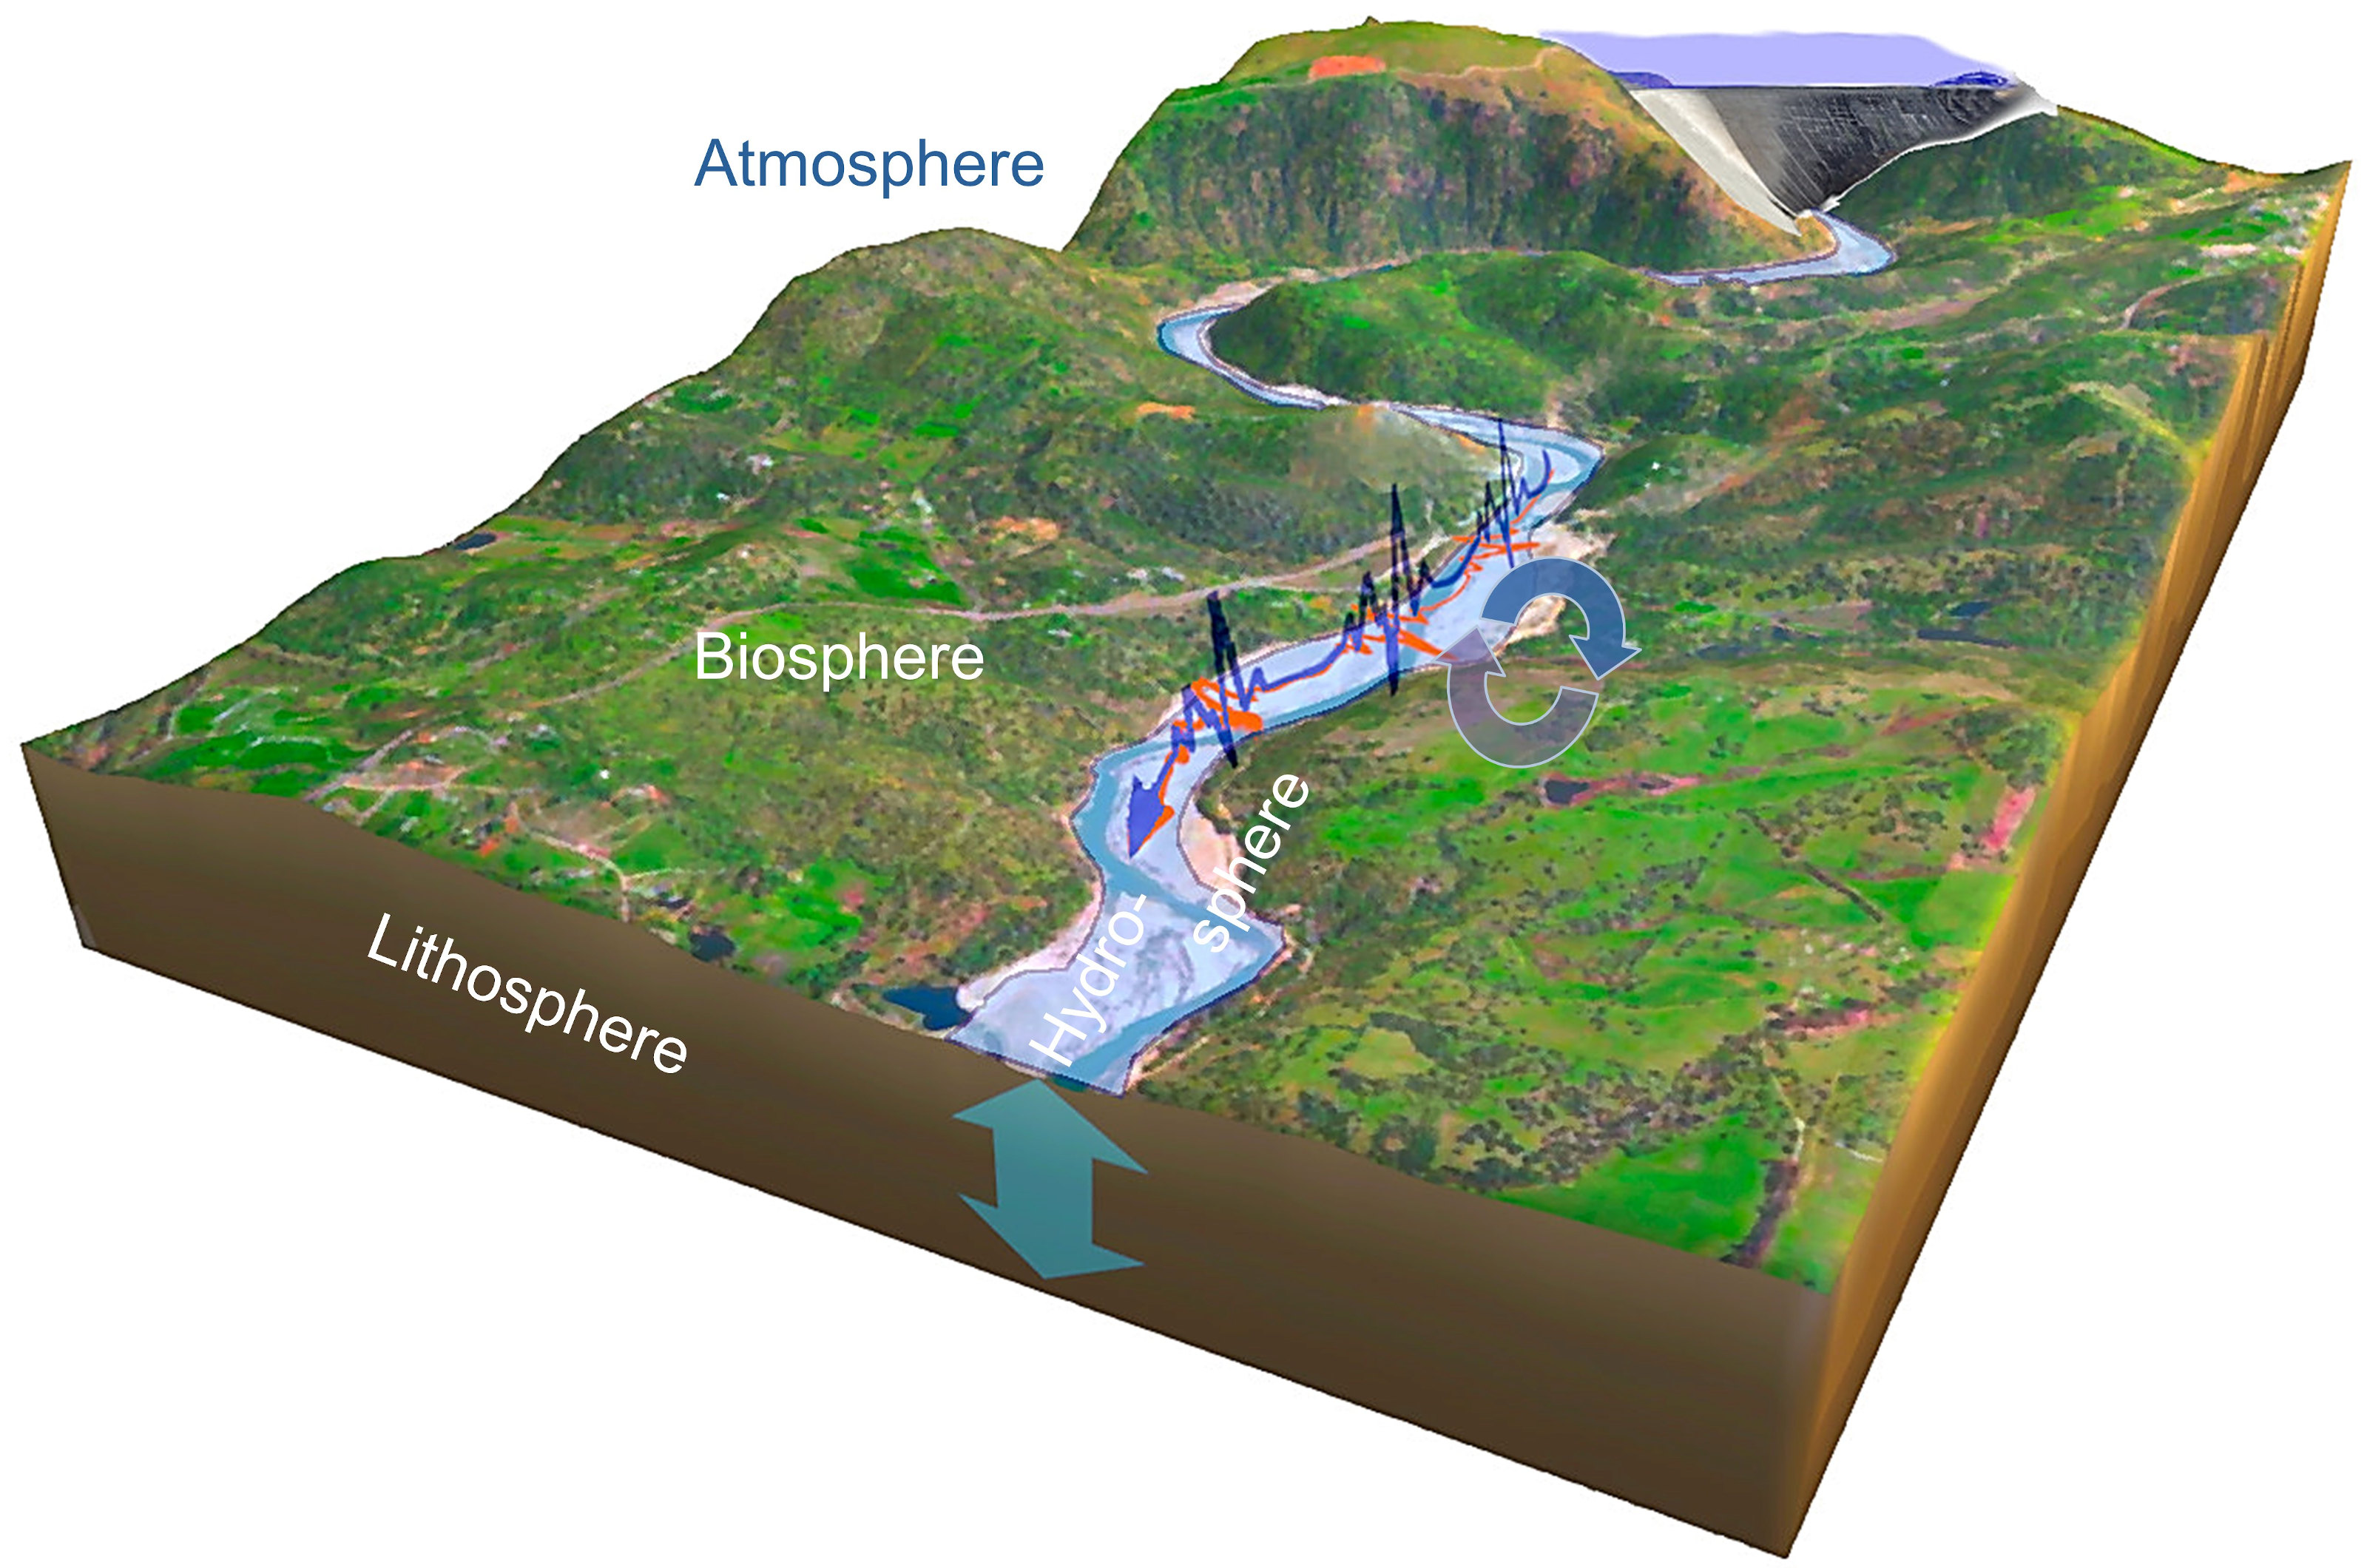
\includegraphics[width=0.82\paperwidth]{hyconnect-with-dam}};
%		\end{scope}}
%		\onslide<1->{
%			\fill[unisblue,opacity=0.7,xshift=-0.91\paperwidth,yshift=0.86] (\paperwidth,0.86\paperheight) circle (0.11\paperheight);
%			% place text in circle
%			\node at (\paperwidth,0.865\paperheight)[xshift=-0.908\paperwidth,yshift=0.865,text width=0.135\paperwidth,align=center]{\bf \large {\textcolor{white}{Spatio-temporal axes}}};
%		}
%	\end{tikzpicture}
%\end{frame}

\subsection{Space \& Time Axes}
\begin{frame}{\secname: \subsecname}
	\begin{tikzpicture}
		\clip (0,0) rectangle (\paperwidth,\paperheight);
		\onslide<1-1>{
			\begin{scope}
				\node[anchor=south west, xshift=0.\paperwidth, yshift=0.2\paperheight] {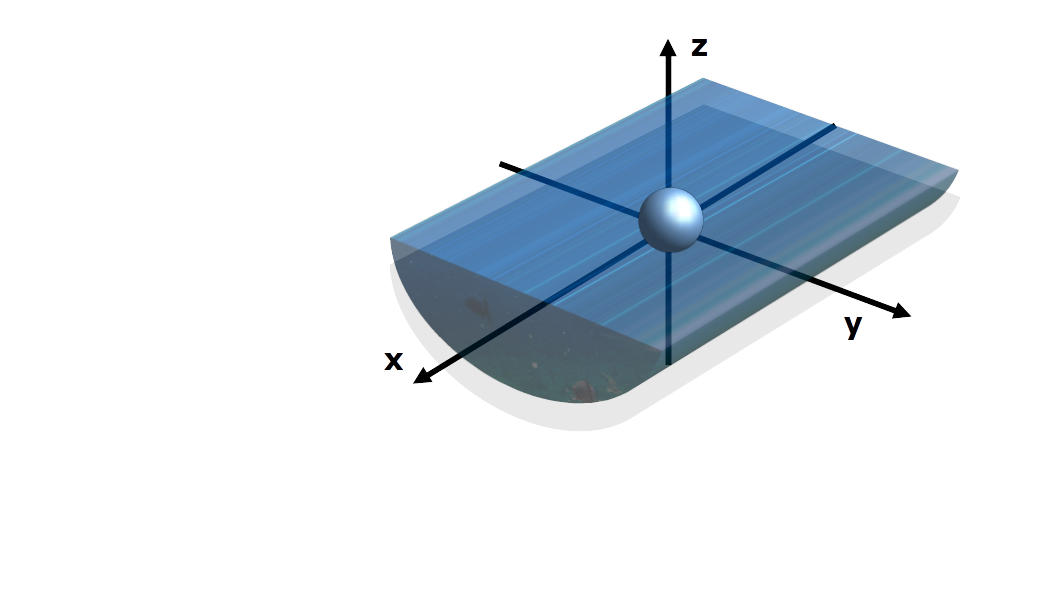
\includegraphics[width=0.9\paperwidth]{connectivity-dimensions-0}};
		\end{scope}}
		\onslide<2->{
			\begin{scope}
				\node[anchor=south west, xshift=0.\paperwidth, yshift=0.2\paperheight] {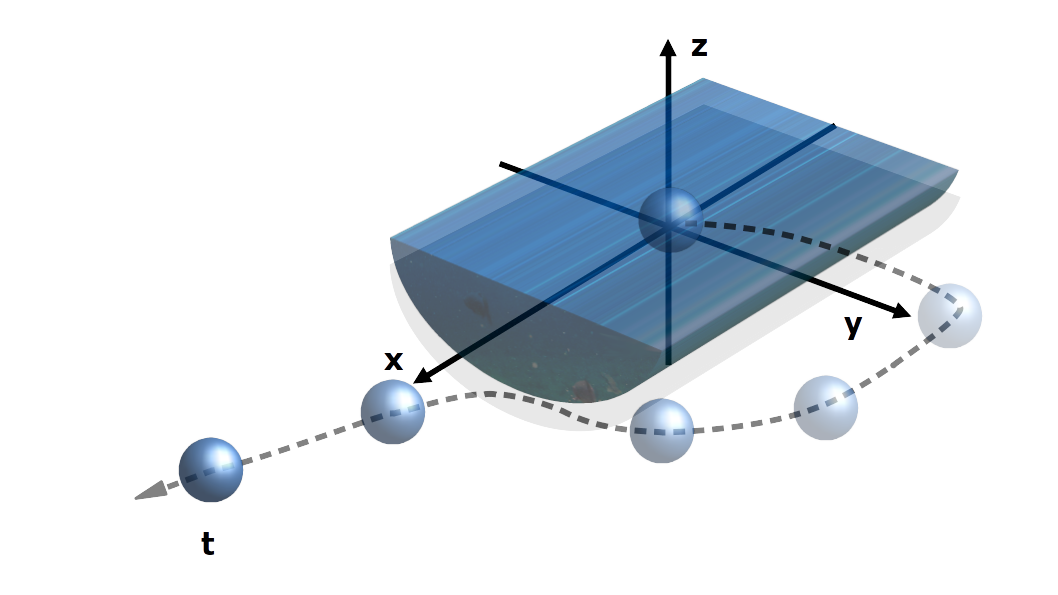
\includegraphics[width=0.9\paperwidth]{connectivity-dimensions-1}};
		\end{scope}}
	\end{tikzpicture}
\end{frame}

\section*{Engineering}
\subsection{Problem \& Solution}
\begin{frame}{\secname: \subsecname}
	\begin{tikzpicture}
		\clip (0,0) rectangle (\paperwidth,\paperheight);
		\onslide<1->{
			\begin{scope}
				\node[anchor=south west, xshift=0.\paperwidth, yshift=0.235\paperheight] {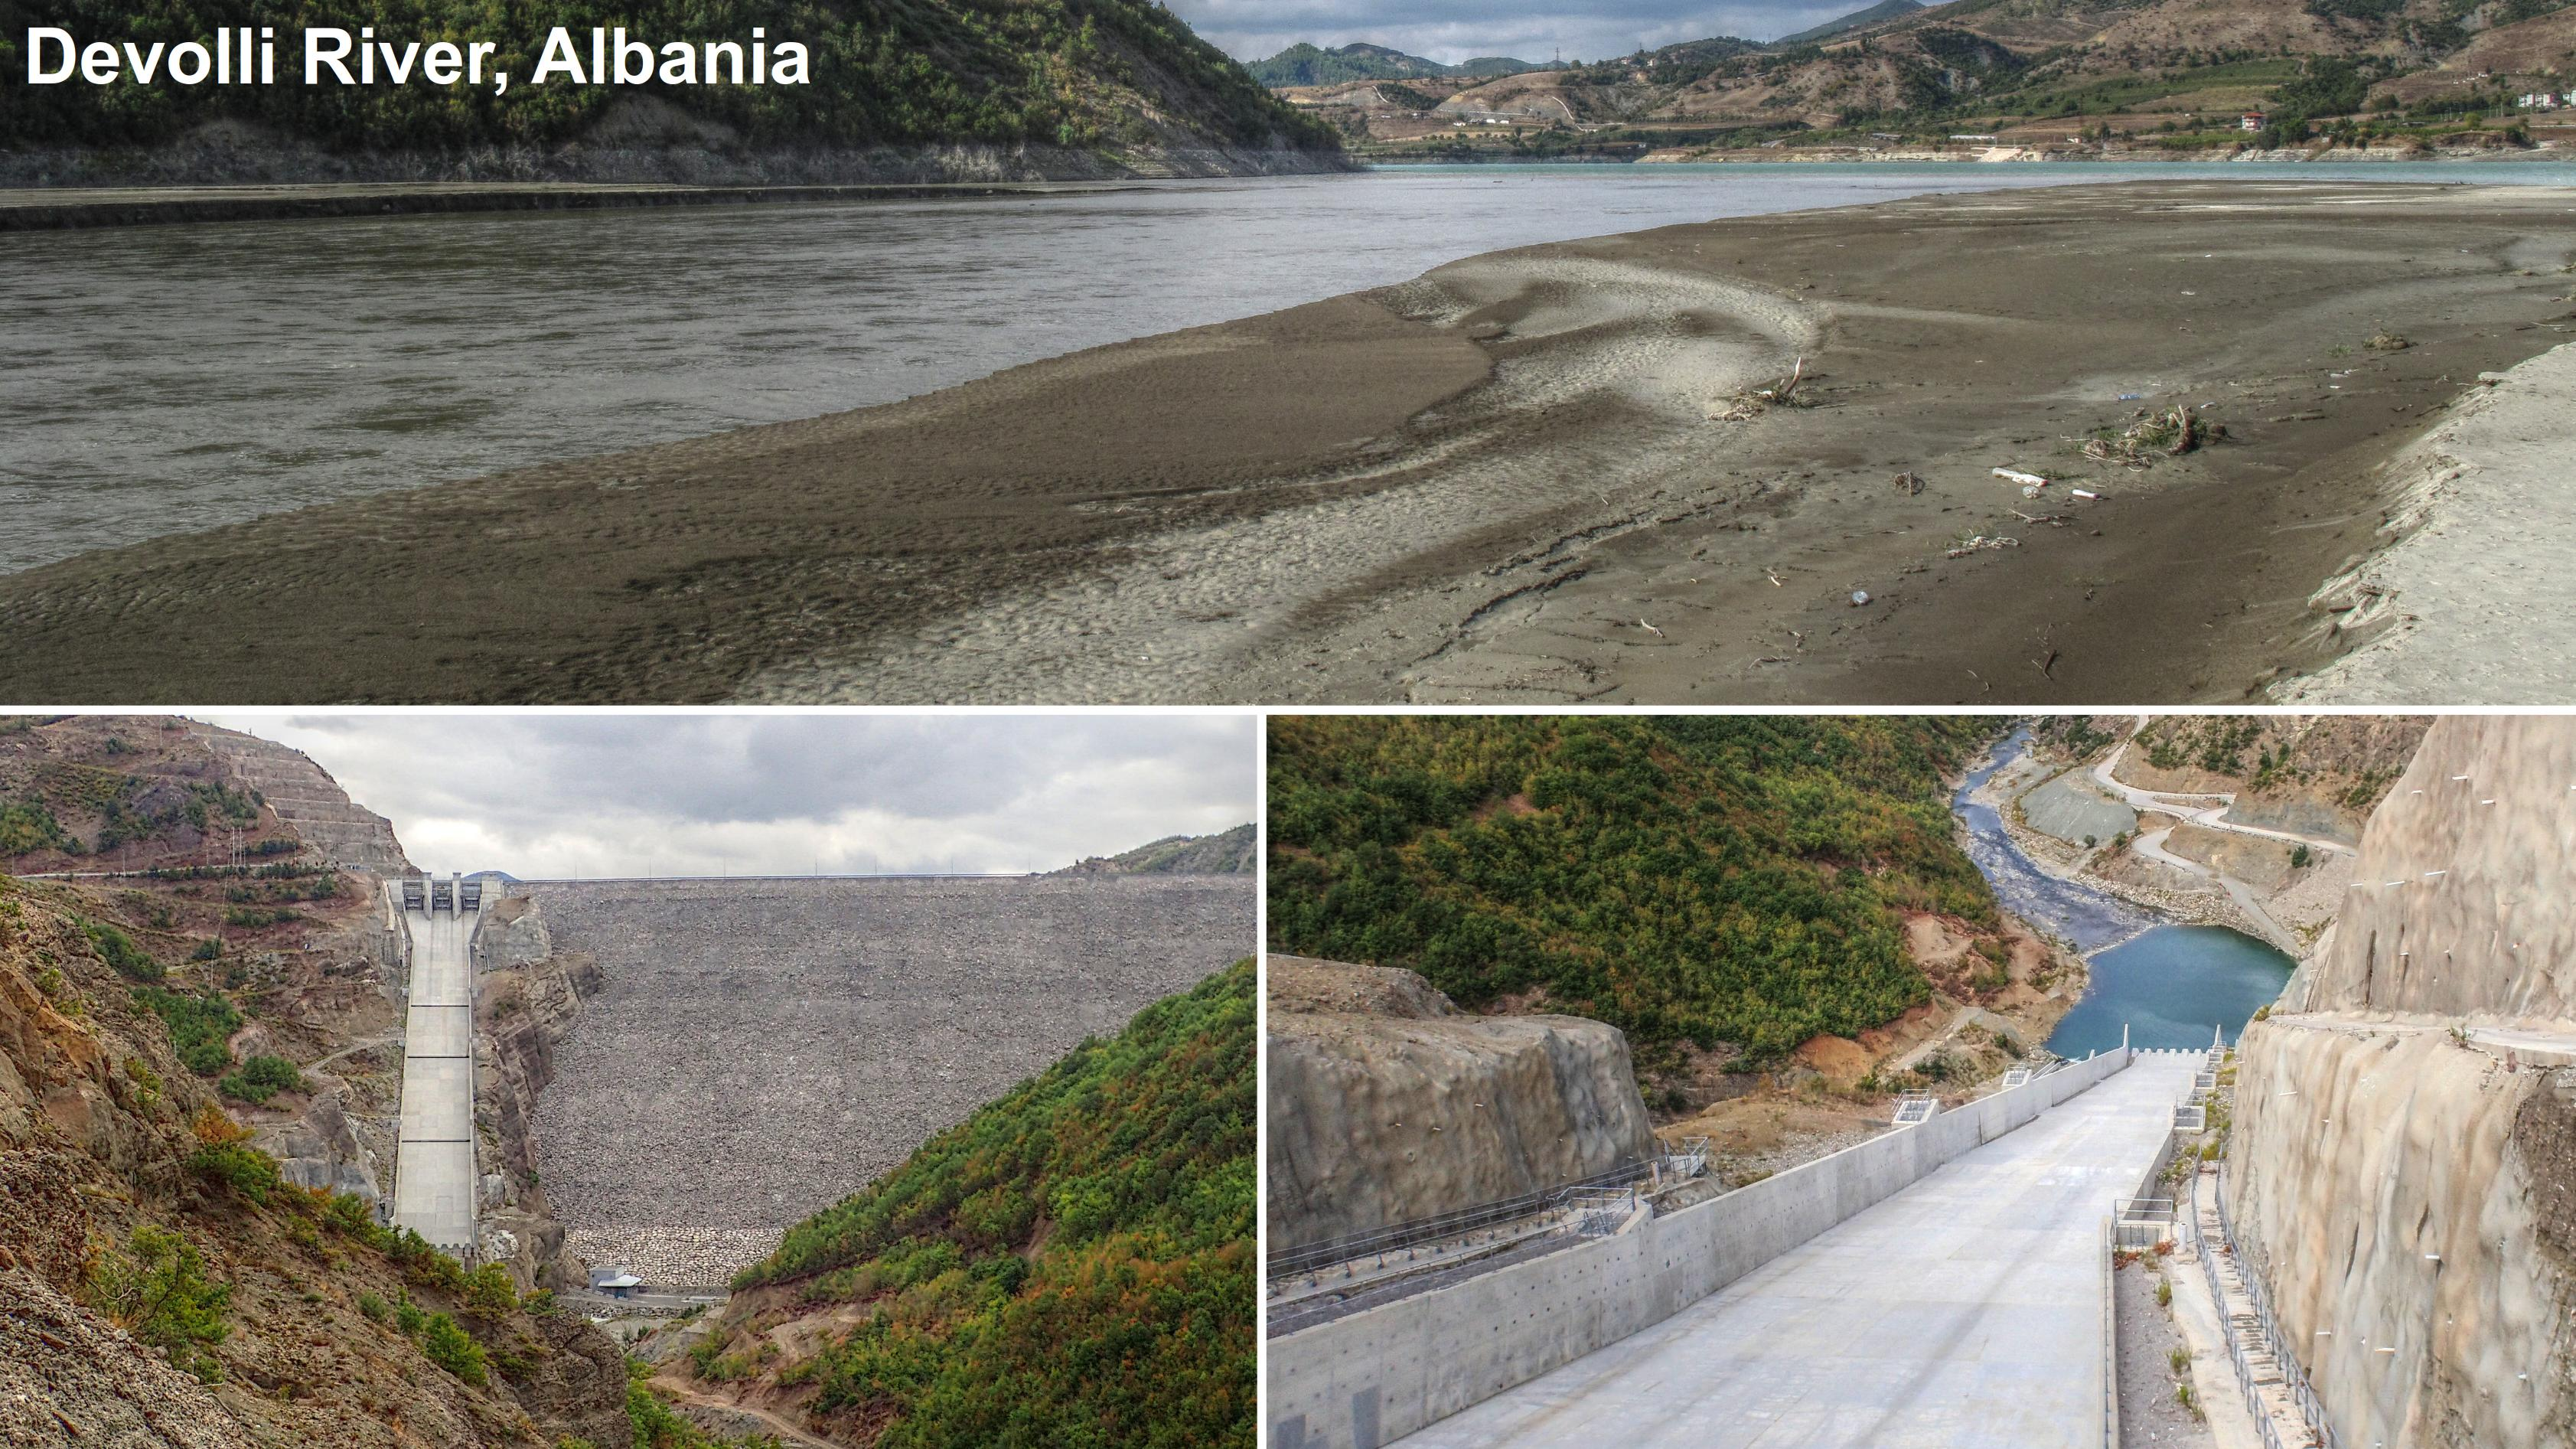
\includegraphics[width=0.88\paperwidth]{engineering-image-assembley}};
		\end{scope}}
		\onslide<2->{
		\begin{scope}
				\node[anchor=south west, xshift=0.03\paperwidth, yshift=0.235\paperheight] {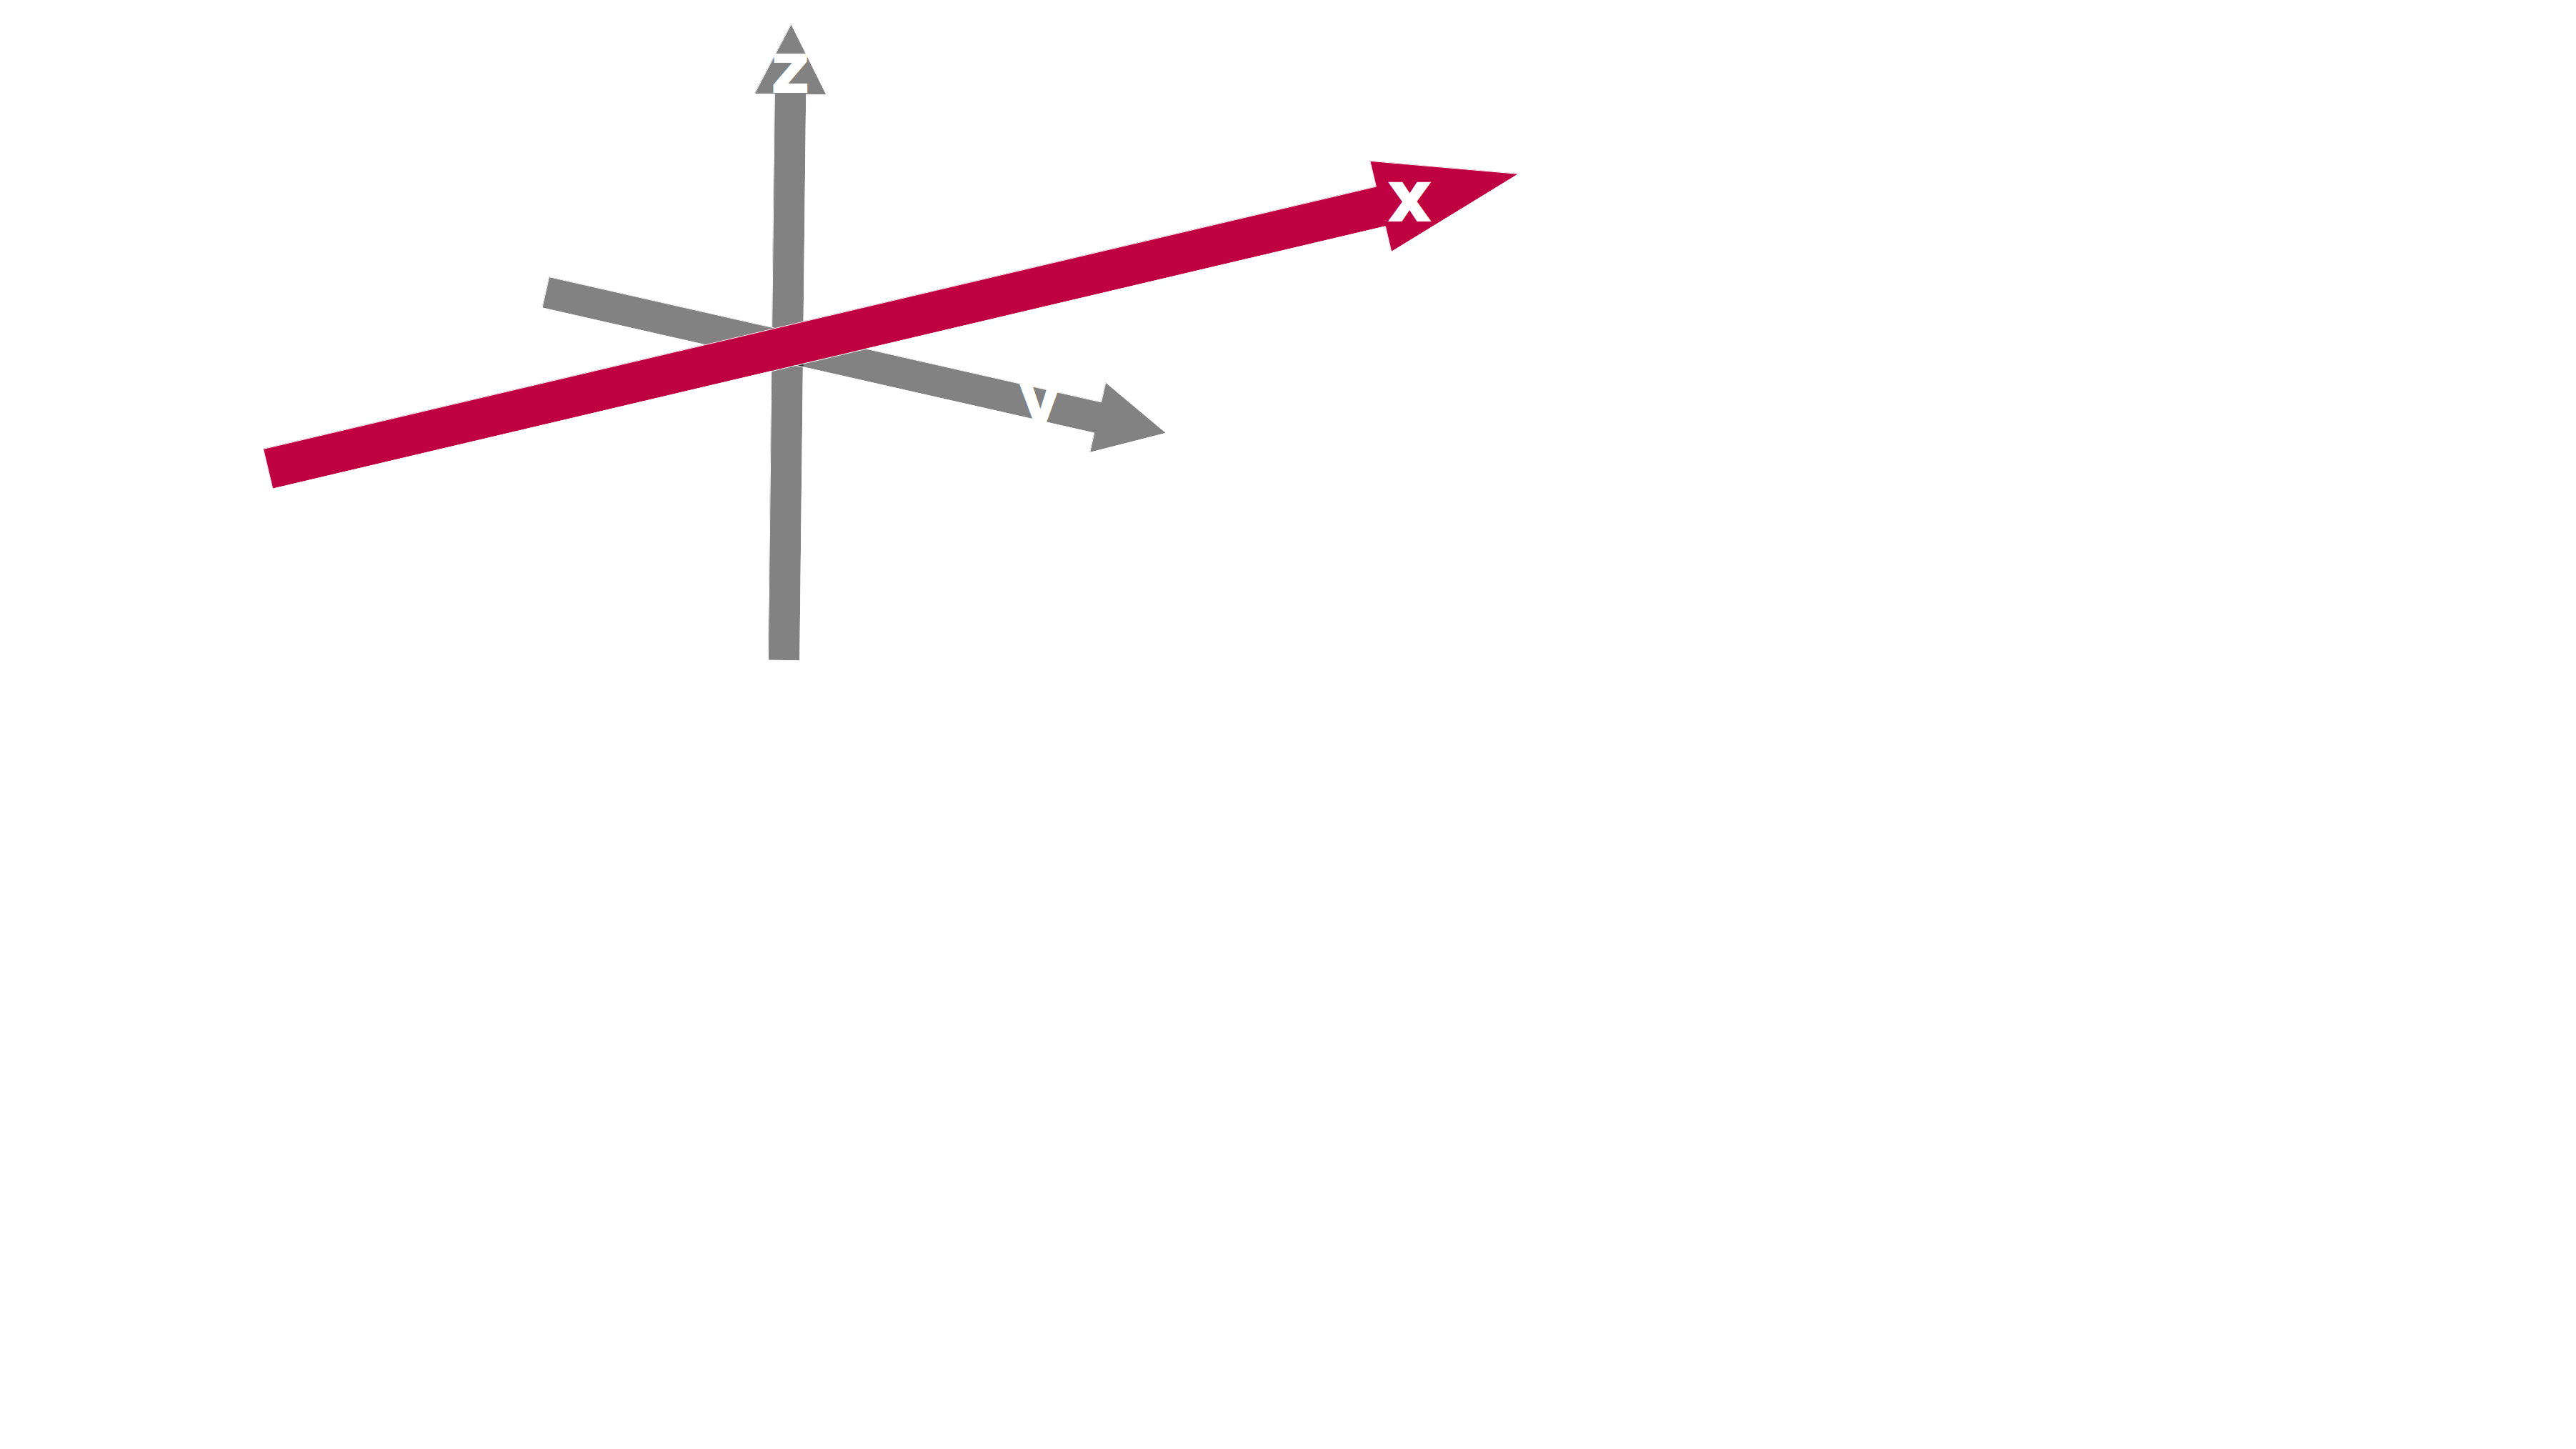
\includegraphics[width=0.88\paperwidth]{engineering-image-assembley-arrows}};
		\end{scope}}
	\end{tikzpicture}
\end{frame}


%\begin{frame}{\secname: \subsecname}
%	\begin{tikzpicture}
%		\clip (0,0) rectangle (\paperwidth,\paperheight);
%		\onslide<1->{
%			\begin{scope}
%				\node[anchor=south west, xshift=0.\paperwidth, yshift=0.235\paperheight] {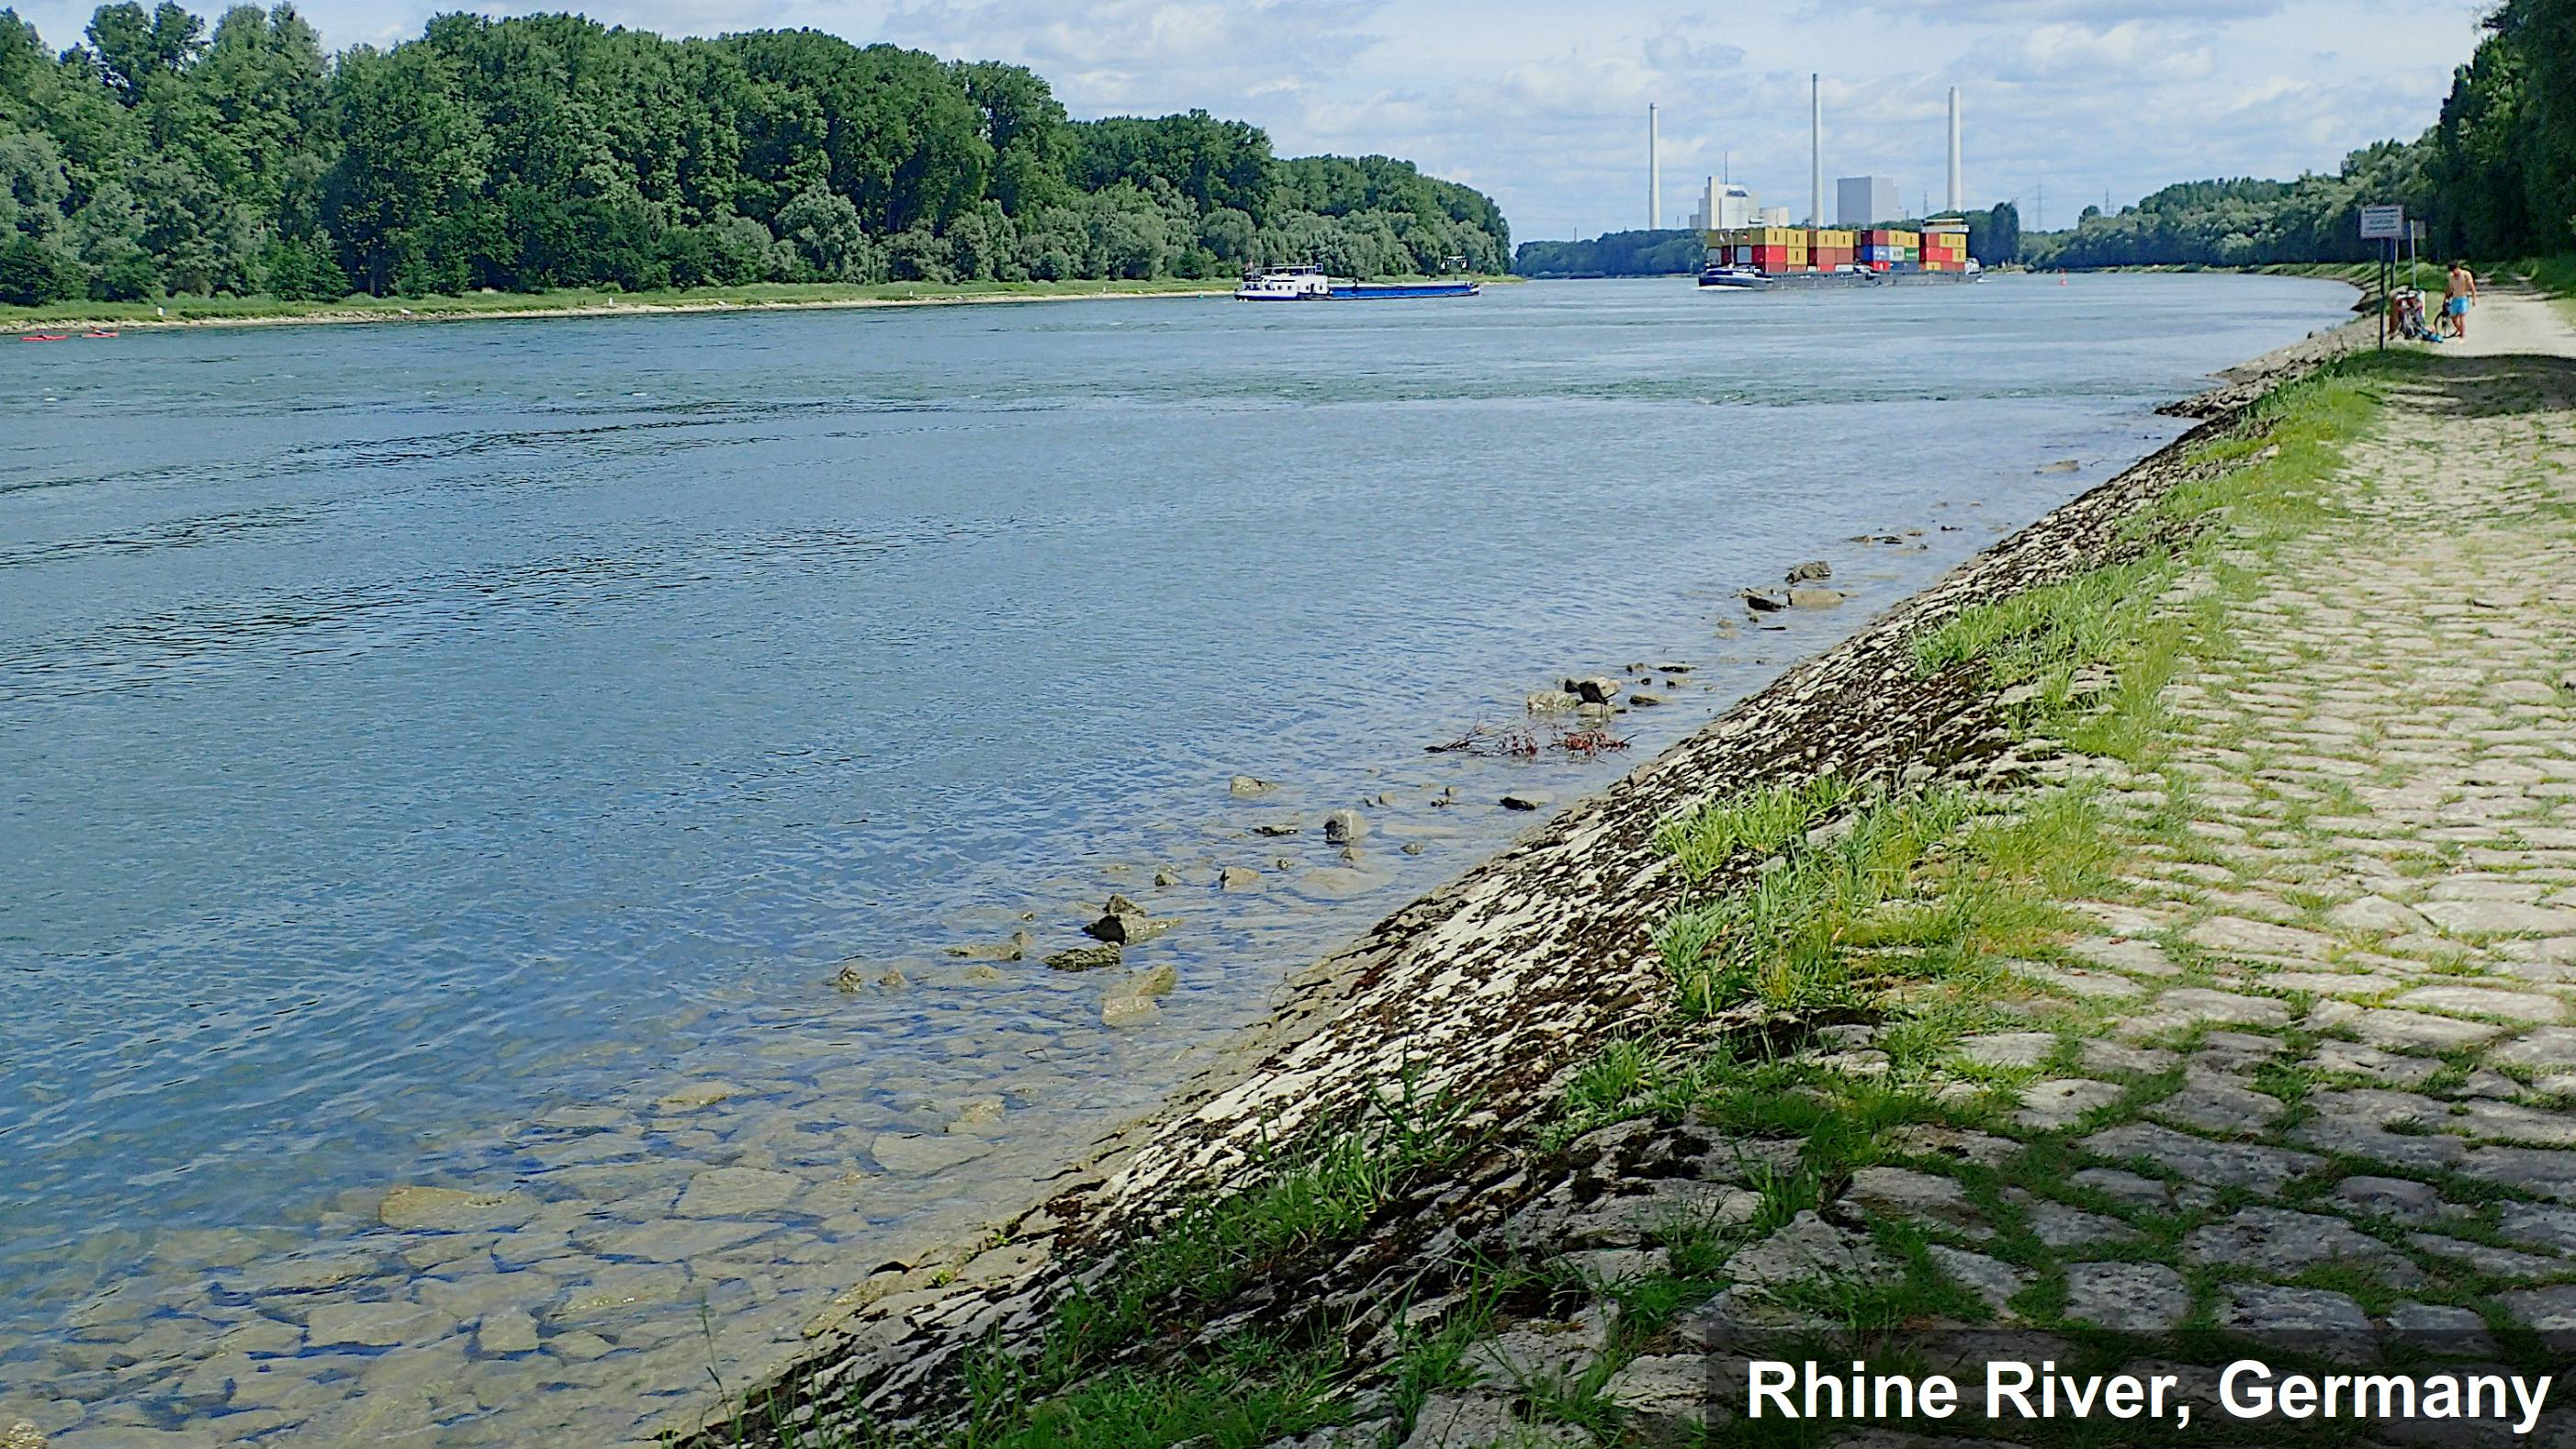
\includegraphics[width=0.88\paperwidth]{rhine-ww}};
%		\end{scope}}
%		\onslide<2->{
%			\begin{scope}
%				\node[anchor=south west, xshift=0.\paperwidth, yshift=0.235\paperheight] {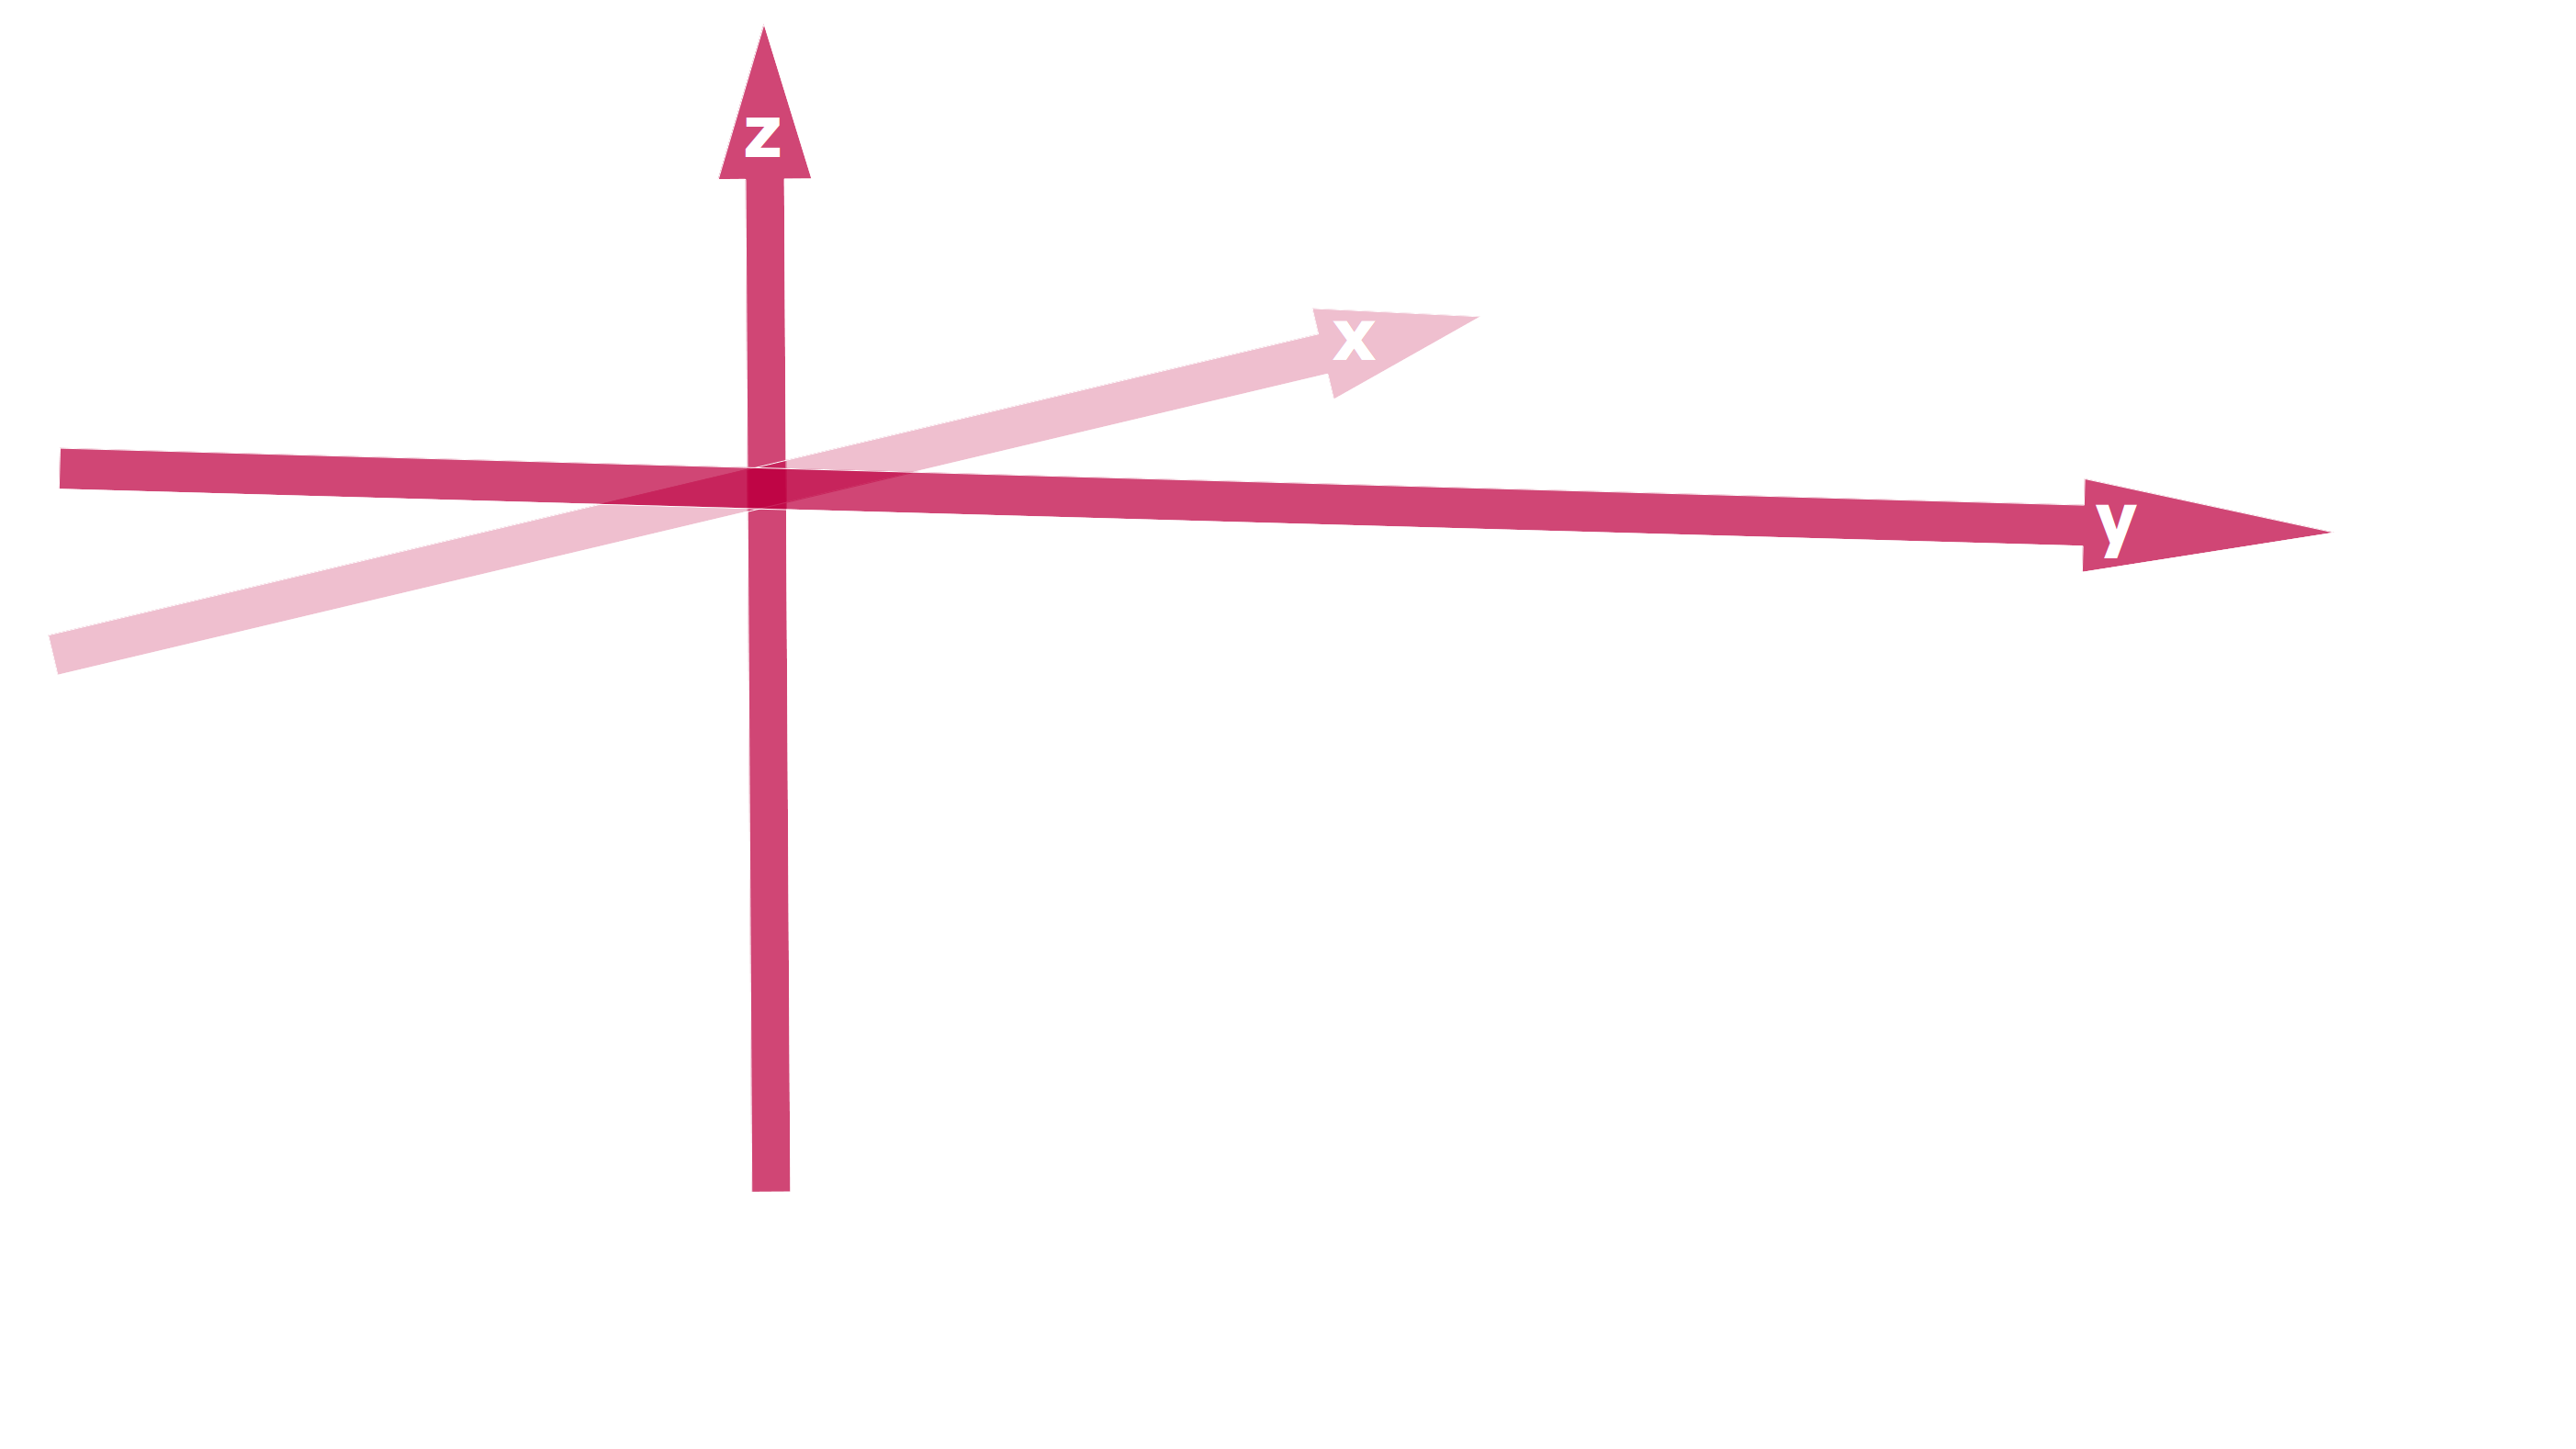
\includegraphics[width=0.88\paperwidth]{rhine-ww-arrows}};
%		\end{scope}}
%	\end{tikzpicture}
%\end{frame}




\begin{frame}{\secname: \subsecname}
	Reconnecting the x-axis: harm vs. utility of dams
	\begin{tikzpicture}
		\clip (0,0) rectangle (\paperwidth,\paperheight);
		\onslide<1->{
		\begin{scope}
				\node[anchor=south west, xshift=0.\paperwidth, yshift=0.235\paperheight] {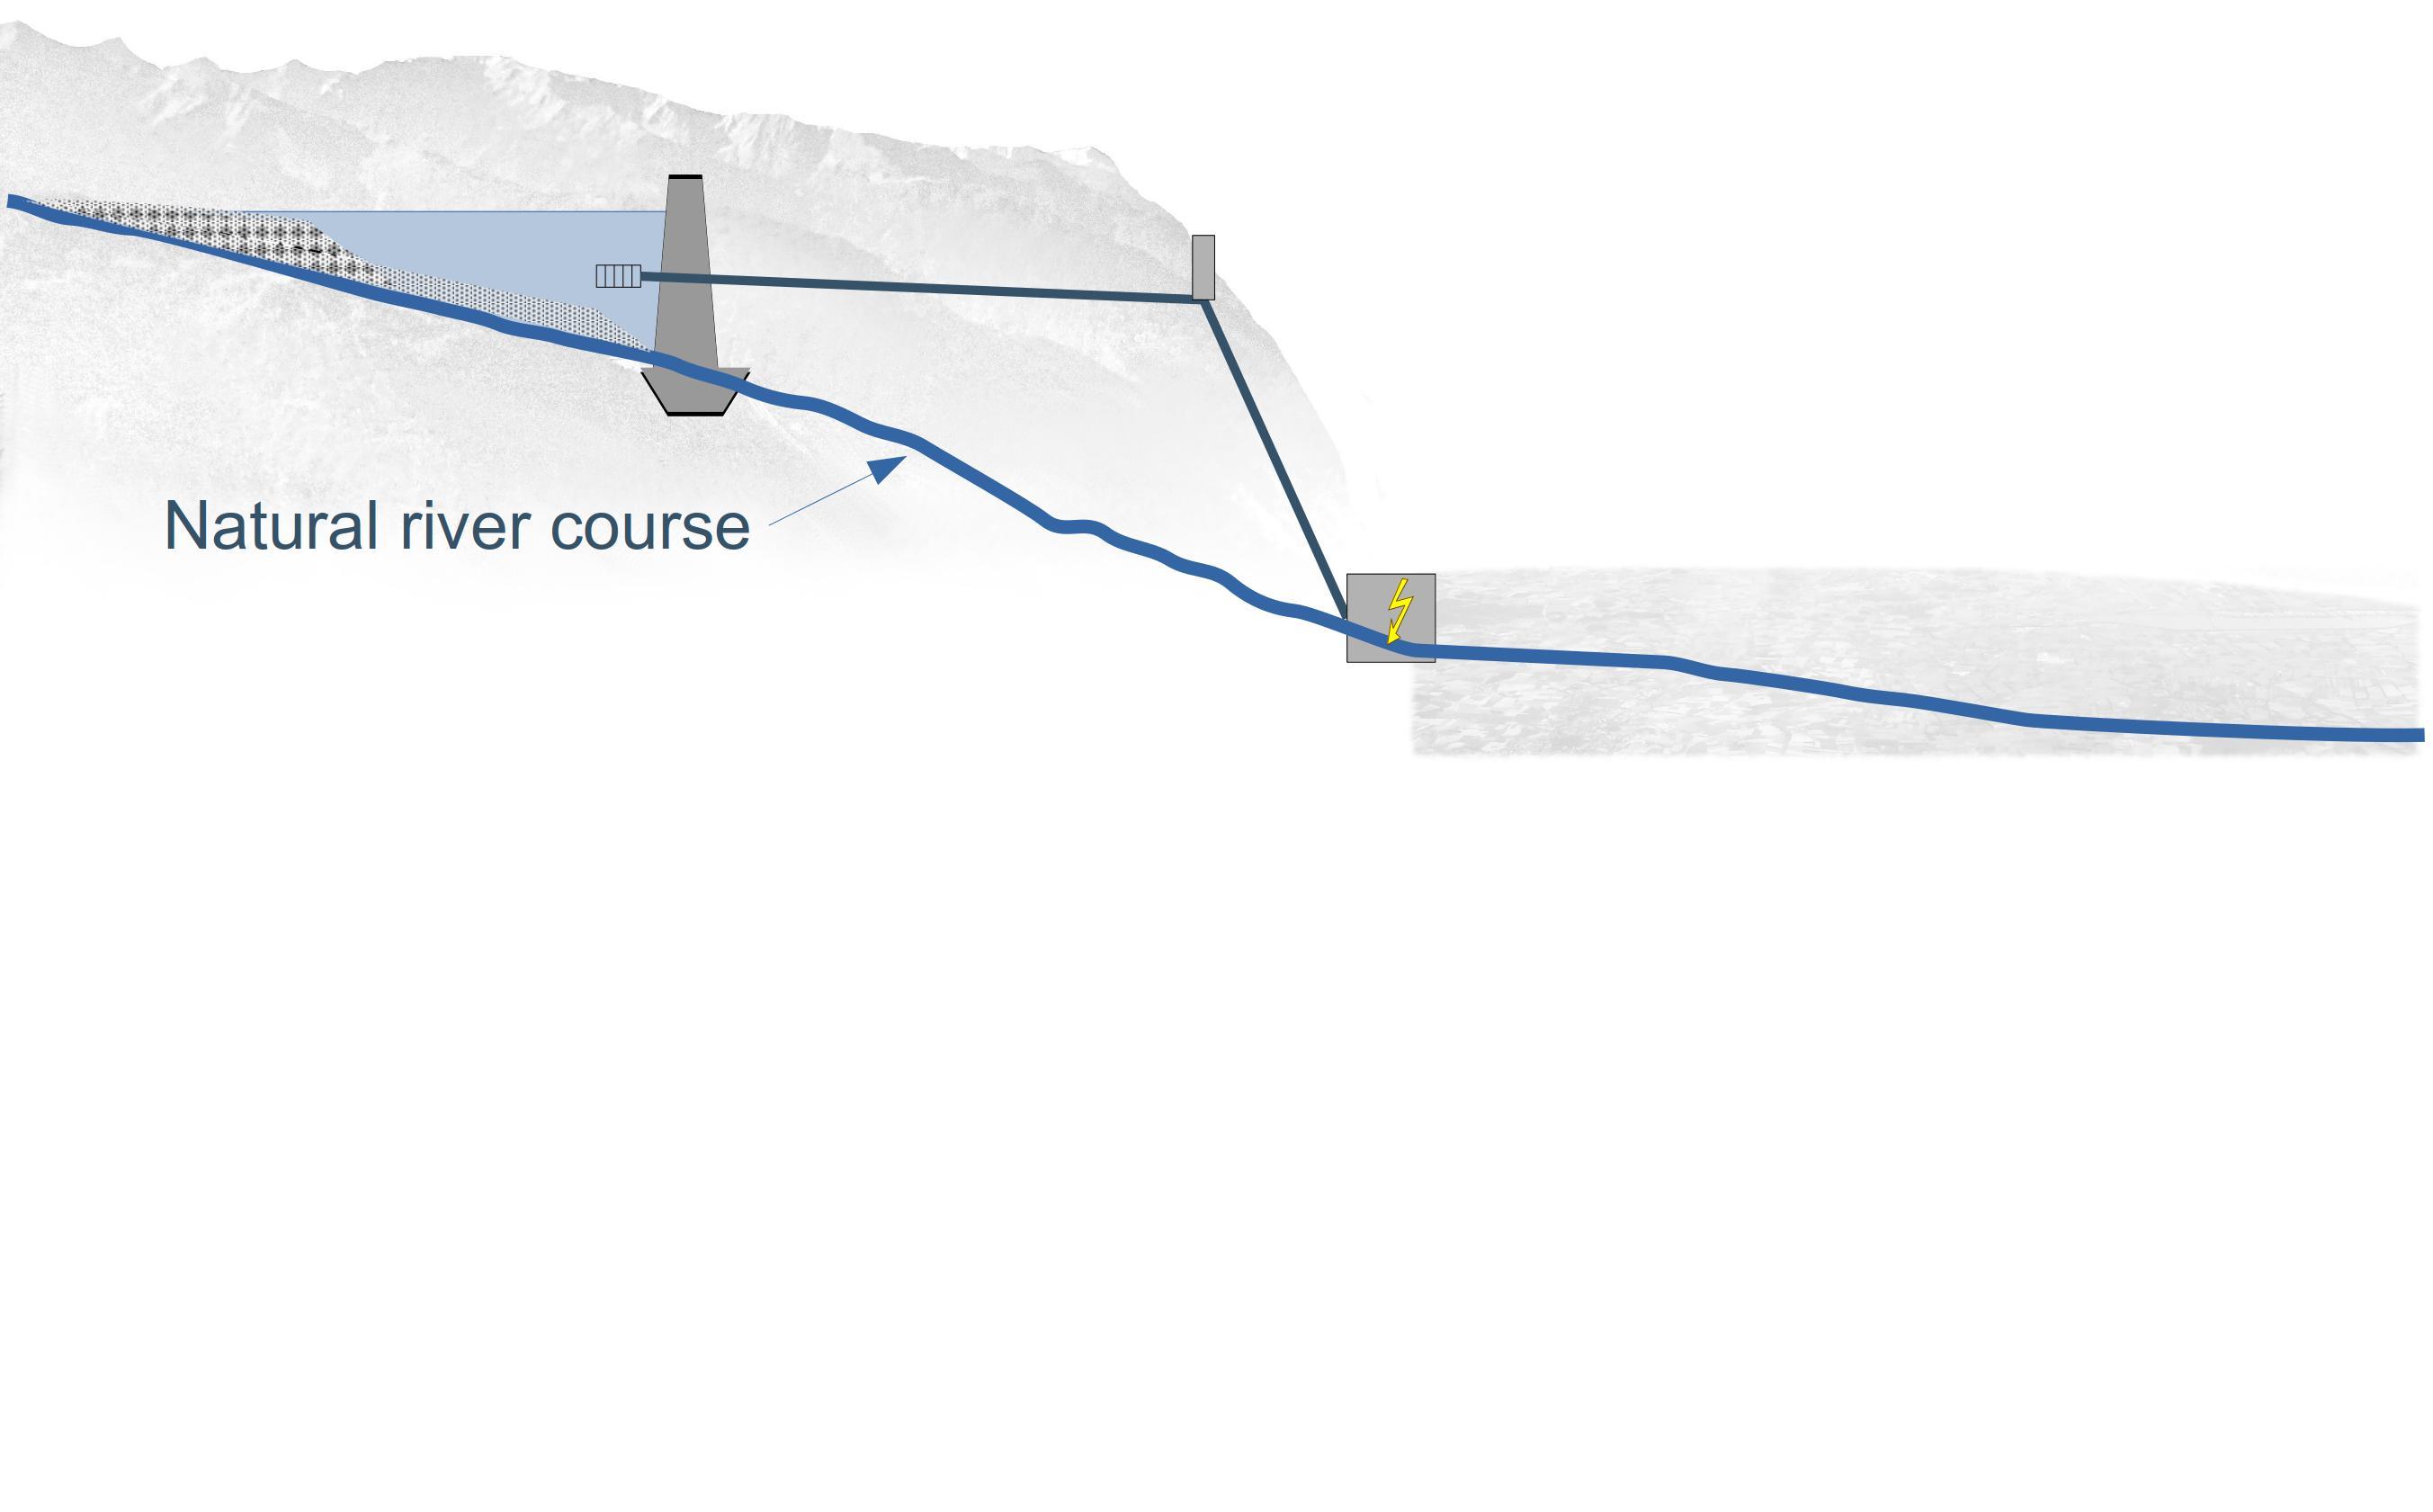
\includegraphics[width=0.88\paperwidth]{dam-scheme-0}};
		\end{scope}}
		\onslide<2->{
			\begin{scope}
				\node[anchor=south west, xshift=0.\paperwidth, yshift=0.235\paperheight] {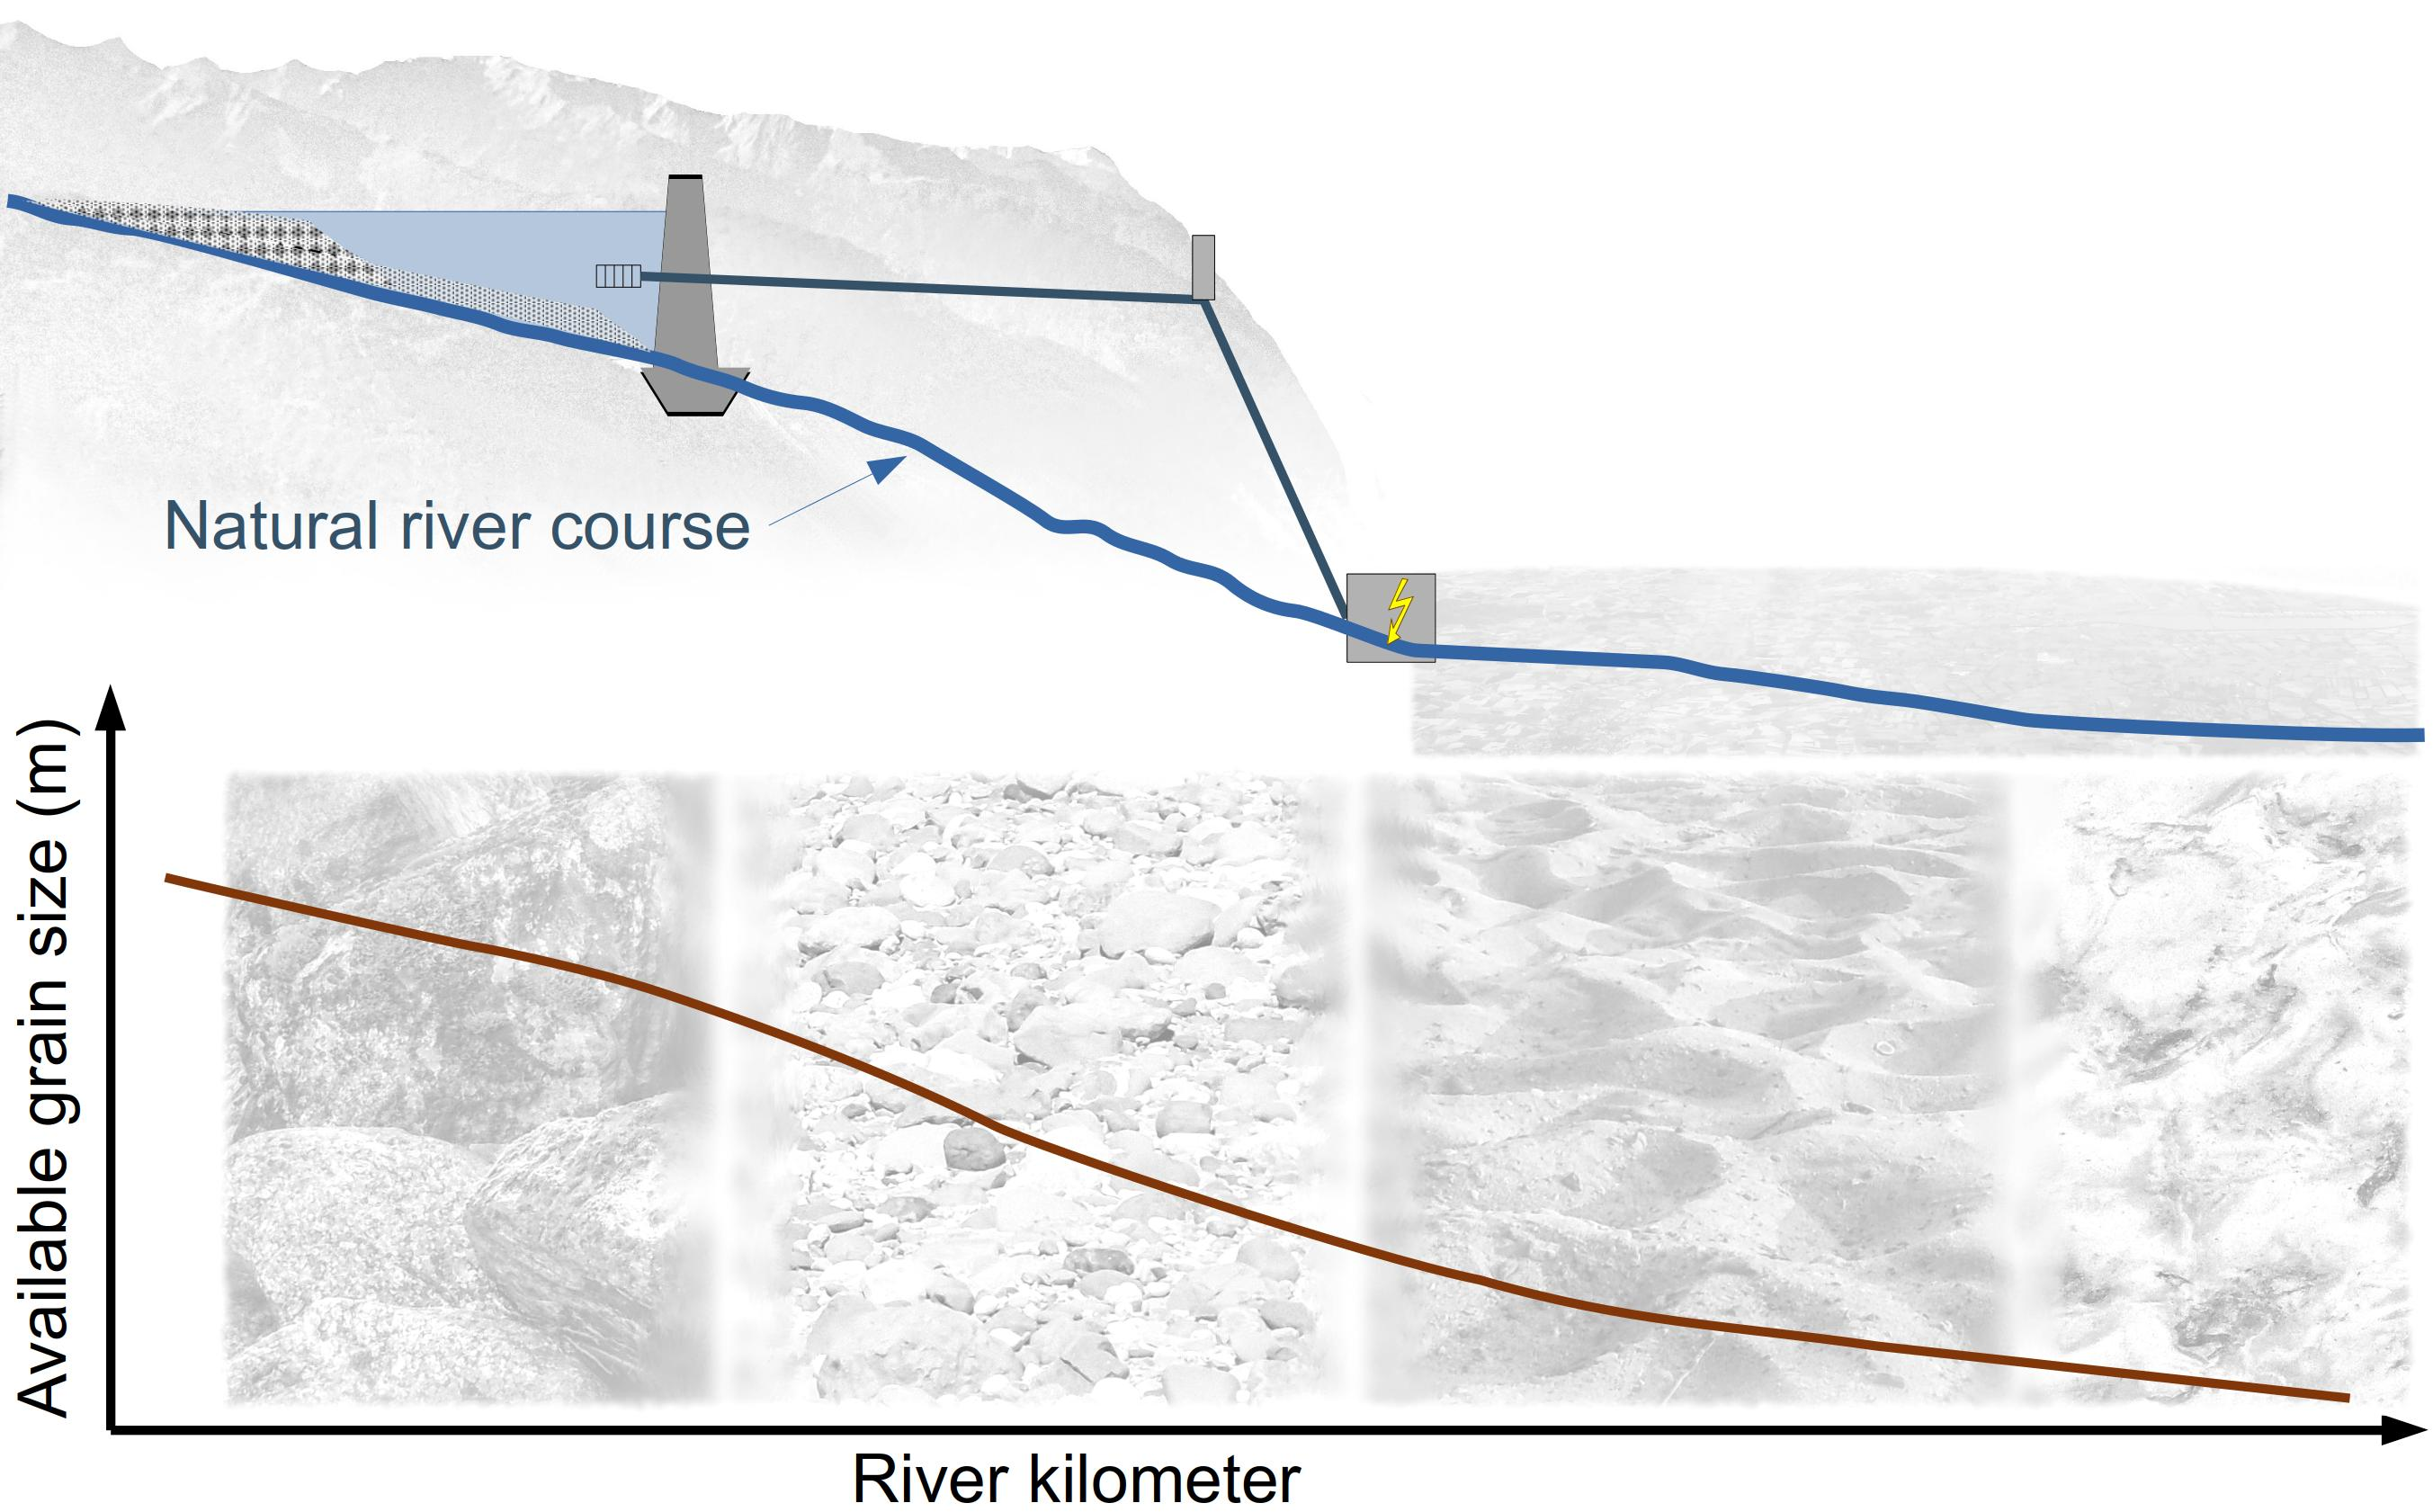
\includegraphics[width=0.88\paperwidth]{dam-scheme-1}};
		\end{scope}}
	\end{tikzpicture}
\end{frame}

%\begin{frame}{\secname: \subsecname}
%	\begin{tikzpicture}
%		\clip (0,0) rectangle (\paperwidth,\paperheight);
%		\onslide<1->{
%		\begin{scope}
%				\node[anchor=south west, xshift=0.\paperwidth, yshift=0.235\paperheight] {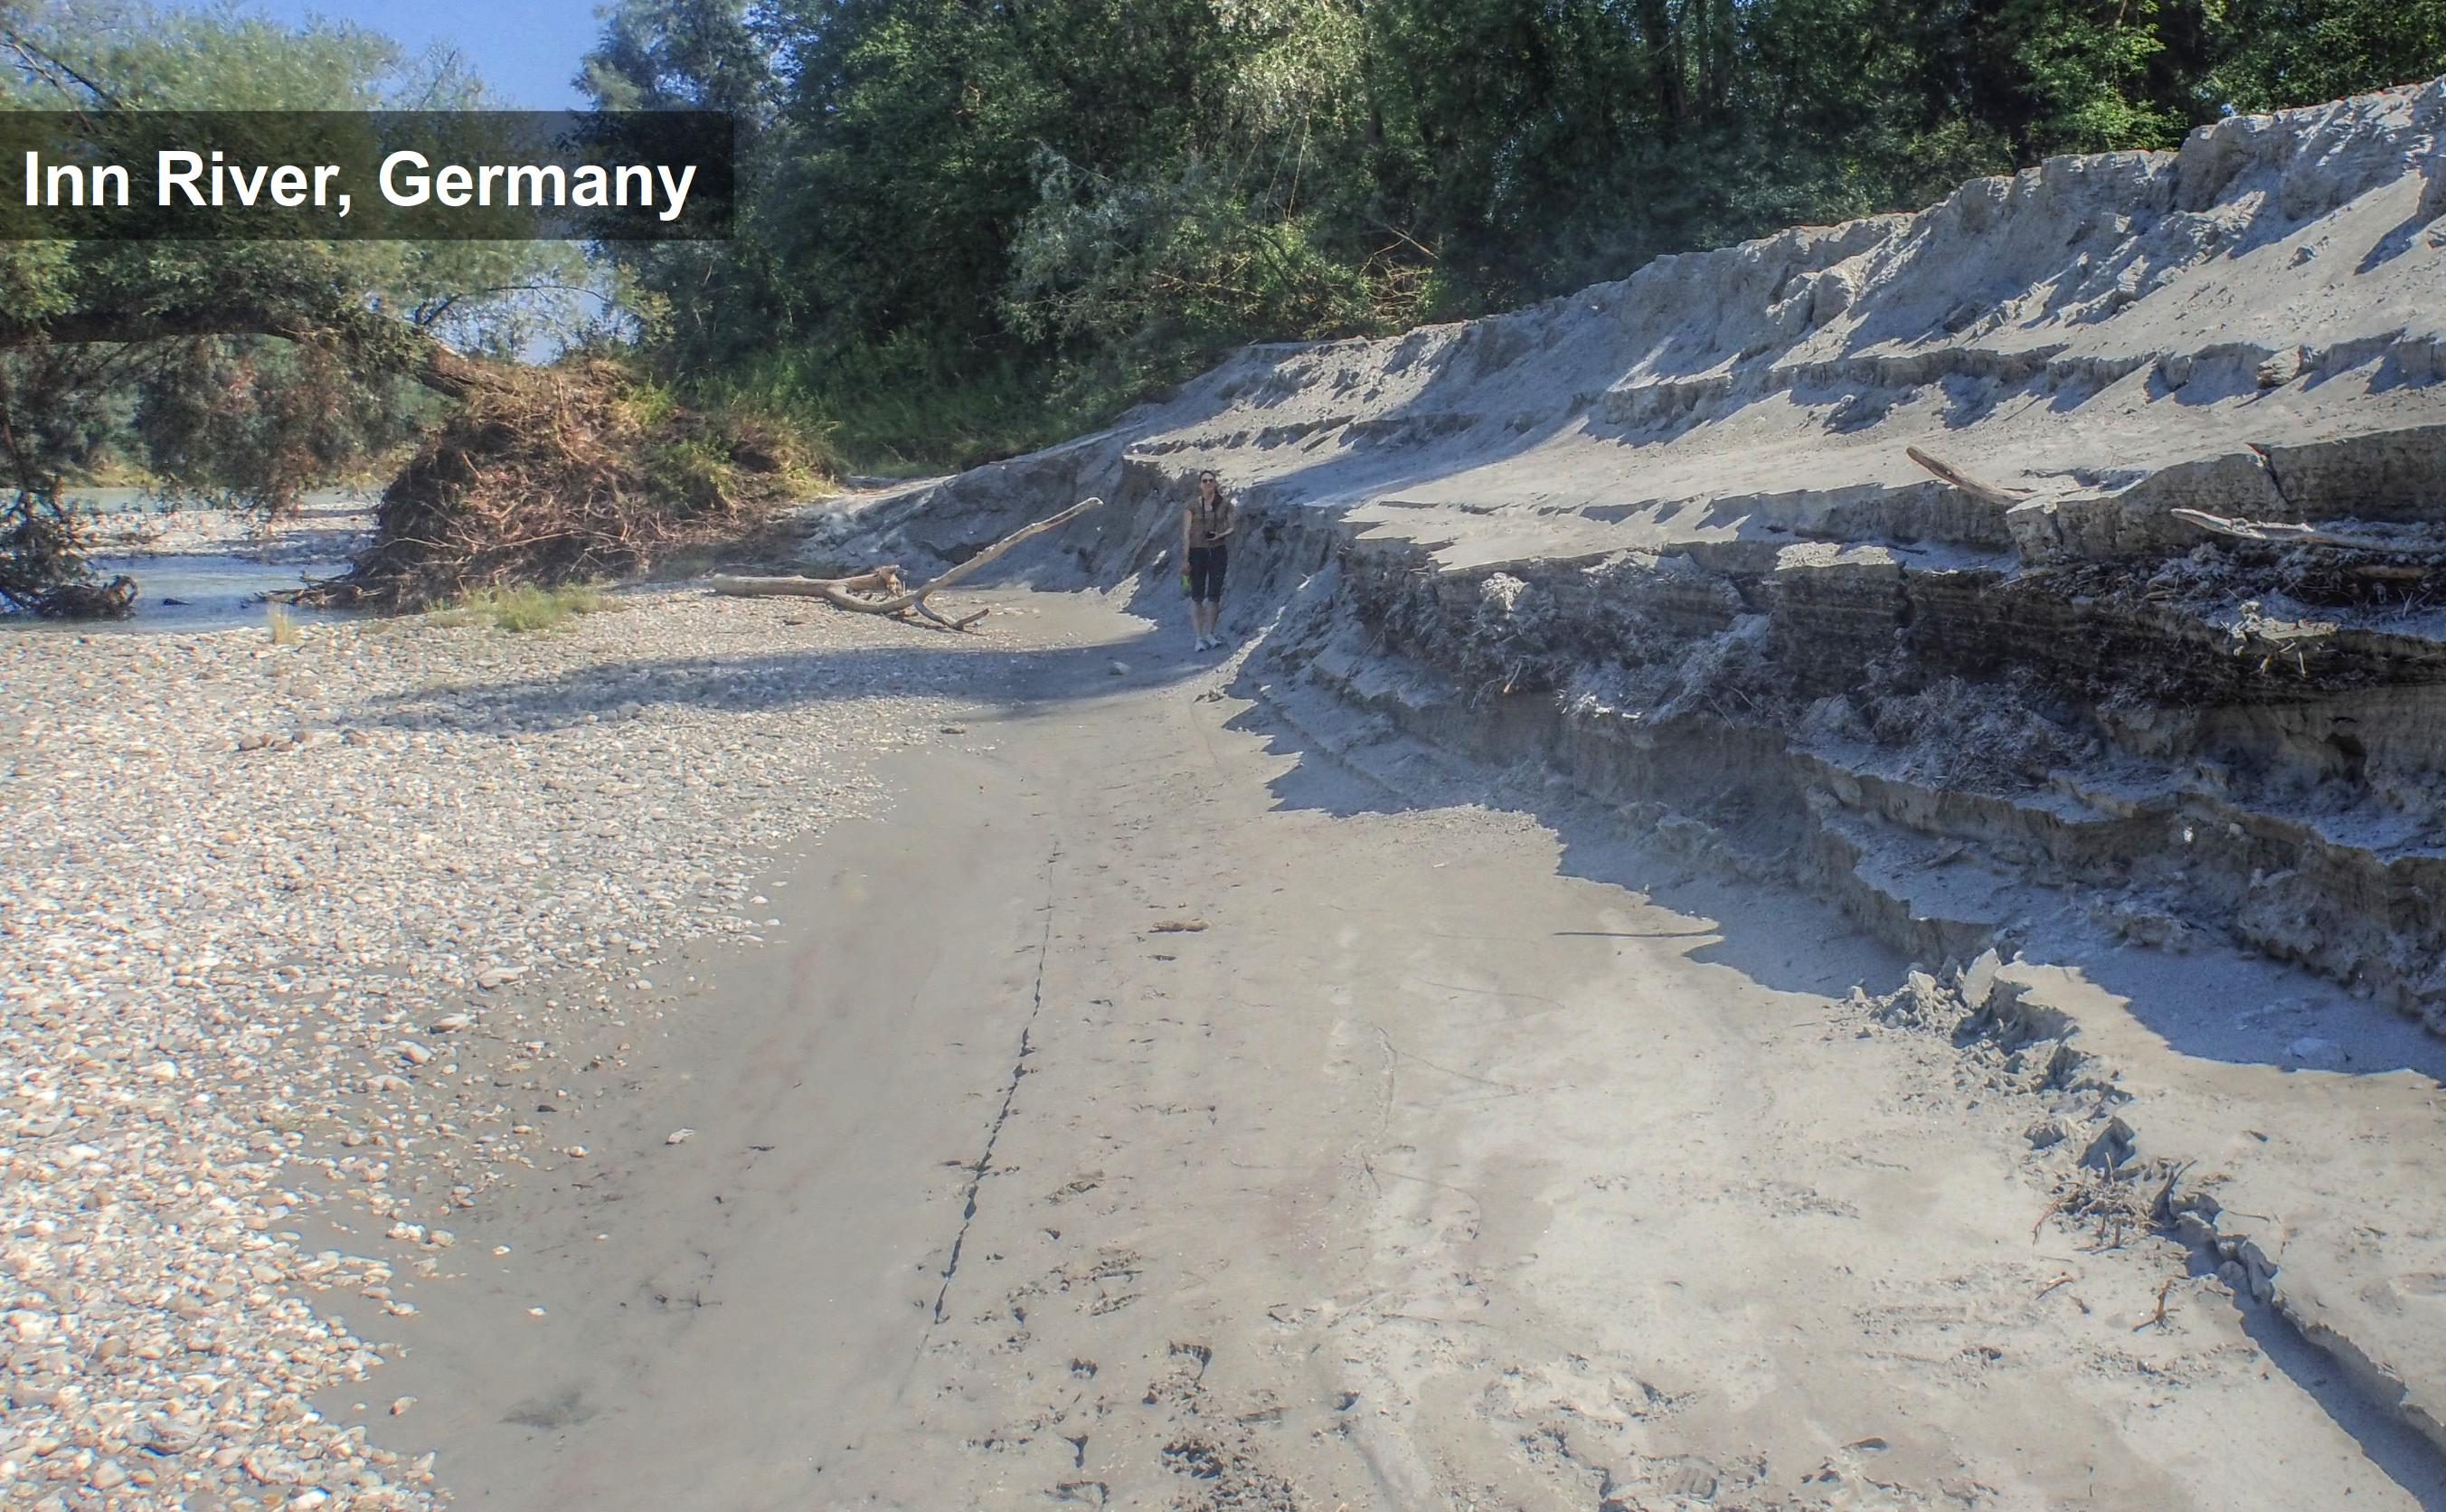
\includegraphics[width=0.88\paperwidth]{inn-sand-bank-ann}};
%		\end{scope}}
%	\end{tikzpicture}
%\end{frame}


{
\usebackgroundtemplate{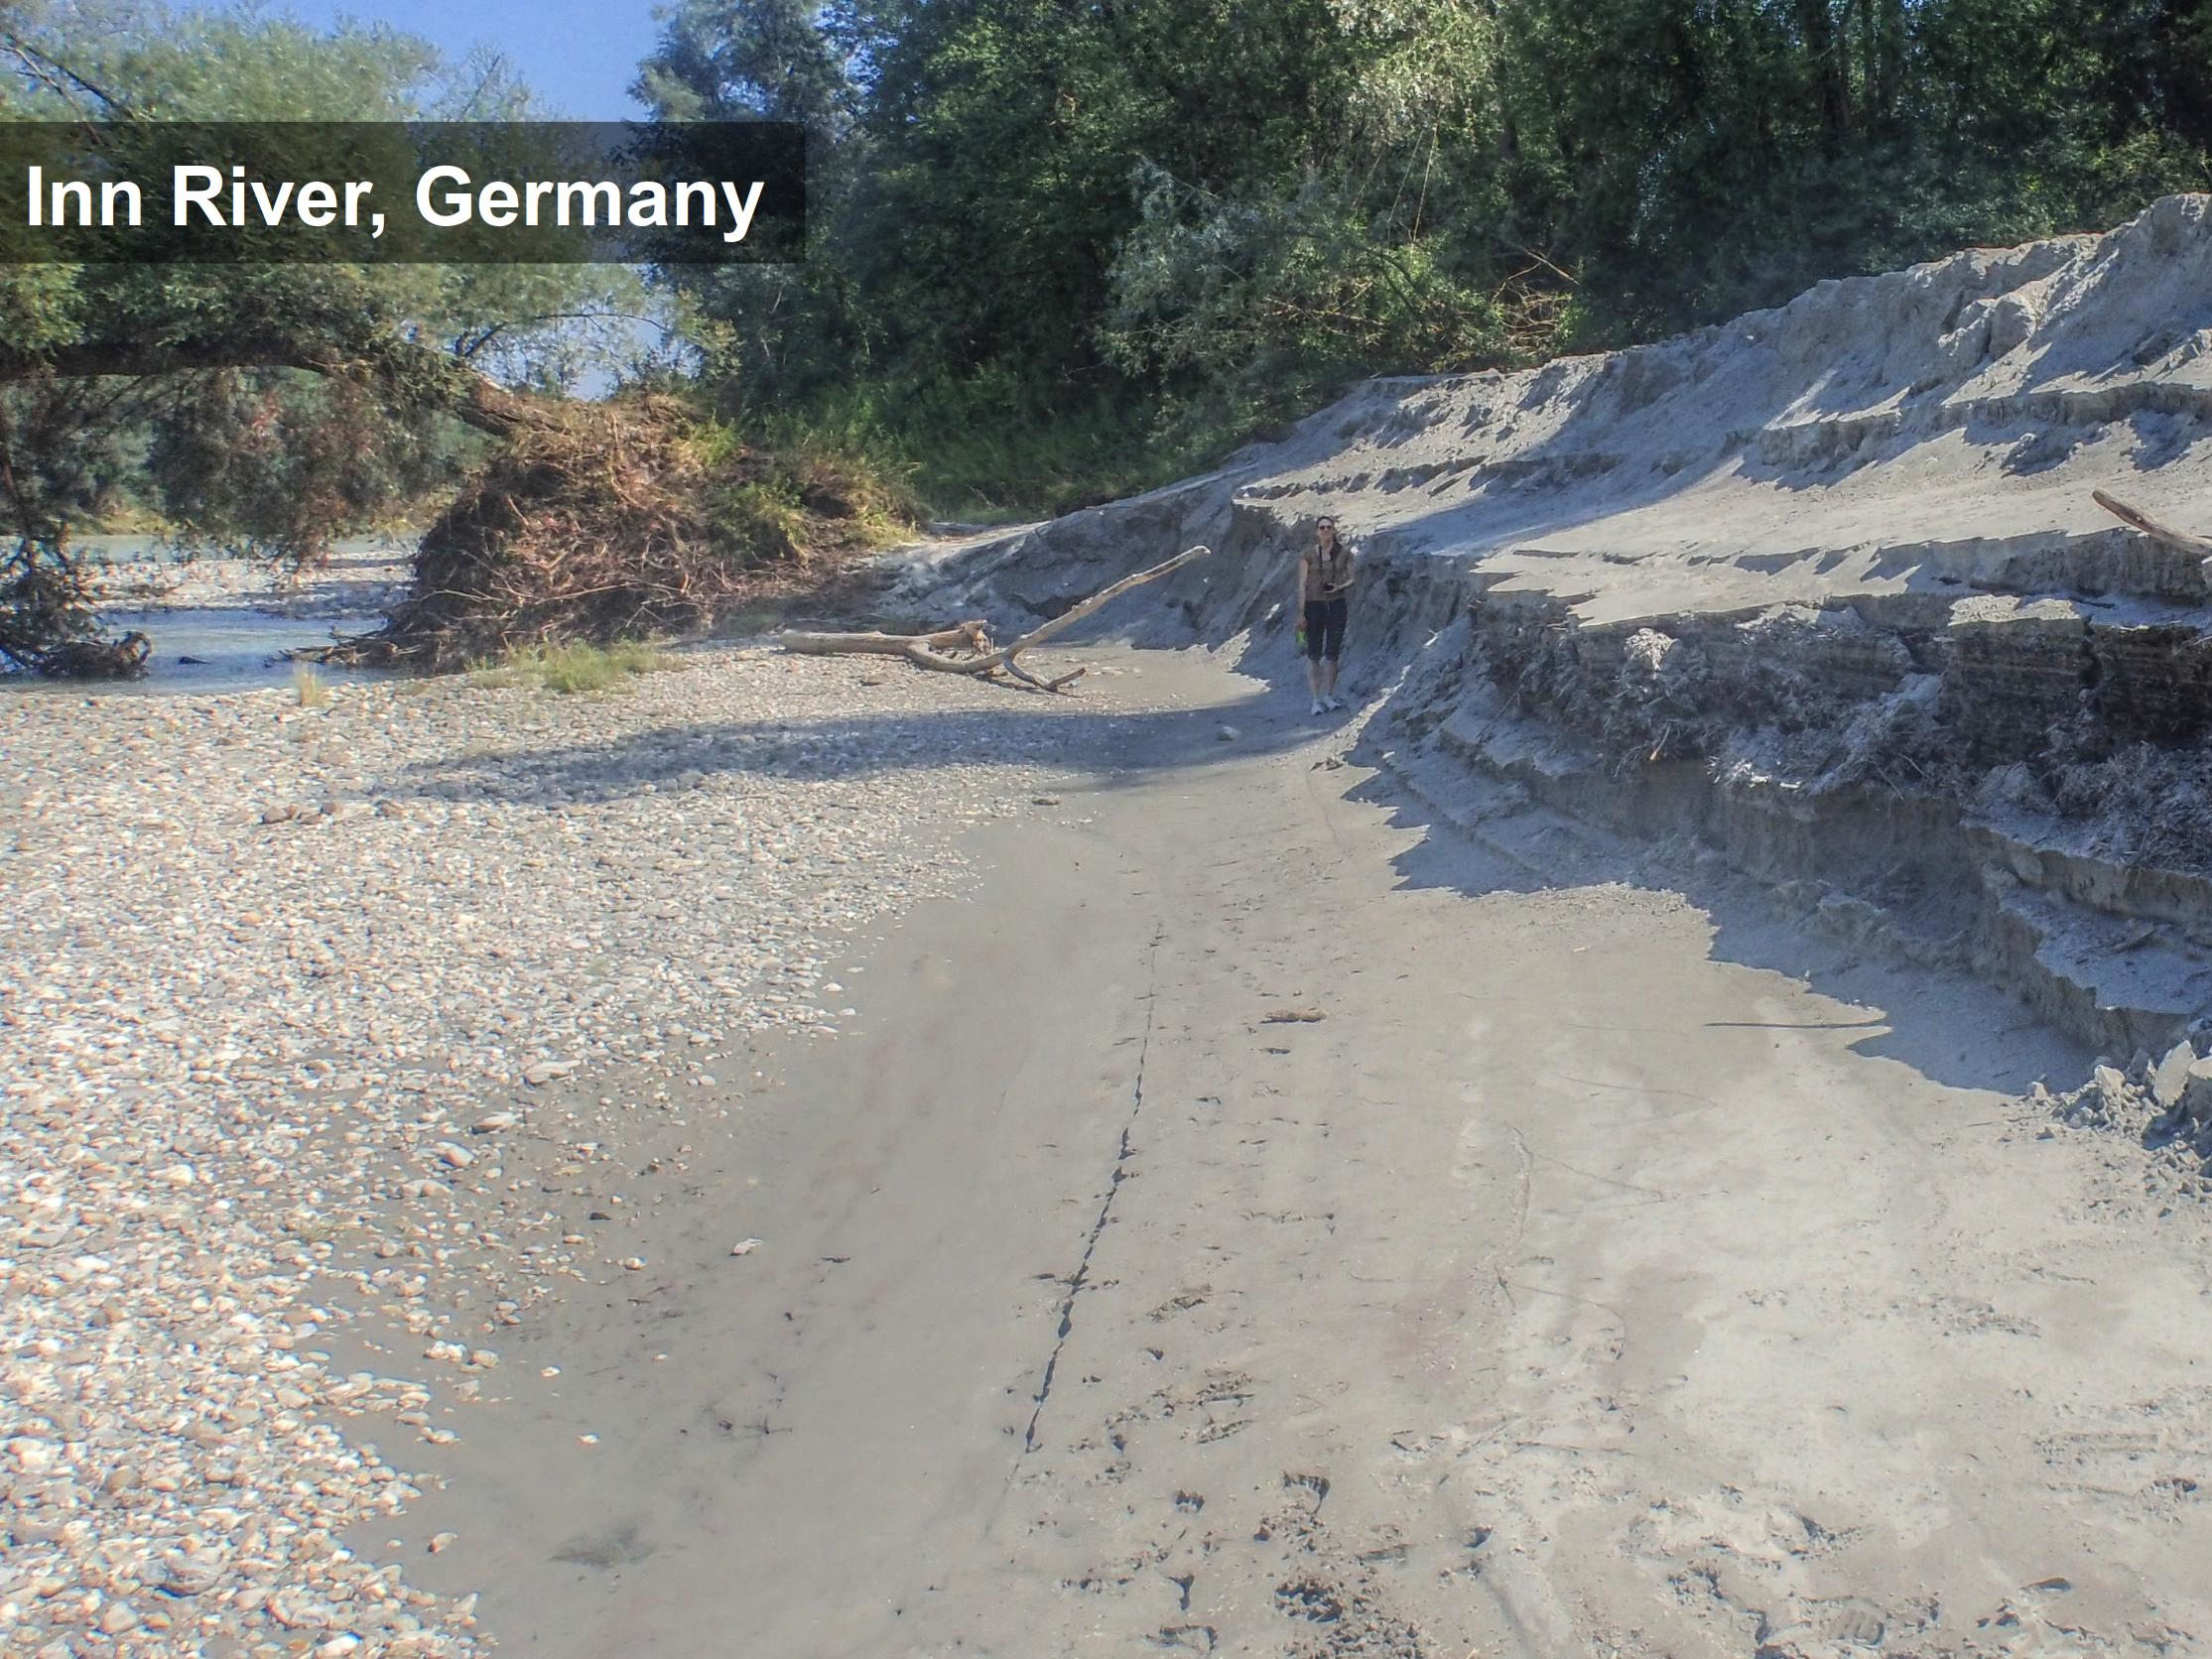
\includegraphics[width=\paperwidth]{inn-sand-bank-ann43.jpg}}%
\begin{frame}[plain]{}{\secname}
	\vspace{3cm}
	\onslide<2->{
	\begin{tcolorbox}[colbacktitle=hellblau!80!black, colback=hellblau!15!white, fonttitle=\bfseries, standard jigsaw,colframe=blue_light, bottom=0mm, middle=0mm, boxsep=0.2mm, opacityframe=0.5, opacityfill=0.75, opacitybacktitle=0.95, title filled, title={Challenges \& Opportunities}, size=fbox]
		\vspace{0.25cm}		 
		\begin{itemize}
			\item[\faChainBroken]\ \textbf{Dams disconnect river ecosystems}
			\item[\faChainBroken]\ No general solution available $\rightarrow$ Local actions\vspace{0.5cm}
			\item[\faChevronCircleRight]\ Optimize actions with fluvial sediment transport assessments
			\item[\faChevronCircleRight]\ Lab \& field data for computer simulations
		\end{itemize}
		\vspace{0.25cm}
	\end{tcolorbox}\smallskip}
\end{frame}}
